%
% Template Laporan Skripsi/Thesis 
%
% @author  Andreas Febrian, Lia Sadita 
% @version 1.03
%
% Dokumen ini dibuat berdasarkan standar IEEE dalam membuat class untuk 
% LaTeX dan konfigurasi LaTeX yang digunakan Fahrurrozi Rahman ketika 
% membuat laporan skripsi. Konfigurasi yang lama telah disesuaikan dengan 
% aturan penulisan thesis yang dikeluarkan UI pada tahun 2008.
%

%
% Tipe dokumen adalah report dengan satu kolom. 
%
\documentclass[12pt, a4paper, onecolumn, oneside, final]{report}

% Load konfigurasi LaTeX untuk tipe laporan thesis
\usepackage{uithesis}
\usepackage{natbib}
\usepackage{import}
\usepackage{url}
% Load konfigurasi khusus untuk laporan yang sedang dibuat
%-----------------------------------------------------------------------------%
% Informasi Mengenai Dokumen
%-----------------------------------------------------------------------------%
% 
% Judul laporan. 
\var{\judul}{Feature Grouping Using Abstract Behavioral Specification Language}
% 
% Tulis kembali judul laporan, kali ini akan diubah menjadi huruf kapital
\Var{\Judul}{FEATURE GROUPING USING ABSTRACT BEHAVIORAL SPECIFICATION LANGUAGE}
% 
% Tulis kembali judul laporan namun dengan bahasa Ingris
\var{\judulInggris}{Feature Grouping Using Abstract Behavioral Specification Language}

% 
% Tipe laporan, dapat berisi Skripsi, Tugas Akhir, Thesis, atau Disertasi
\var{\type}{Proposal Tesis}
% 
% Tulis kembali tipe laporan, kali ini akan diubah menjadi huruf kapital
\Var{\Type}{PROPOSAL TESIS}
% 
% Tulis nama penulis 
\var{\penulis}{Reza Mauliadi}
% 
% Tulis kembali nama penulis, kali ini akan diubah menjadi huruf kapital
\Var{\Penulis}{REZA MAULIADI}
% 
% Tulis NPM penulis
\var{\npm}{1506782404}
% 
% Tuliskan Fakultas dimana penulis berada
\Var{\Fakultas}{ILMU KOMPUTER}
\var{\fakultas}{Ilmu Komputer}
% 
% Tuliskan Program Studi yang diambil penulis
\Var{\Program}{MAGISTER ILMU KOMPUTER}
\var{\program}{Magister Ilmu Komputer}
\var{\programEng}{Master of Computer Science}
% 
% Tuliskan tahun publikasi laporan
\Var{\bulanTahun}{Juni 2016}
% 
% Tuliskan gelar yang akan diperoleh dengan menyerahkan laporan ini
\var{\gelar}{Magister Ilmu Komputer}
% 
% Tuliskan tanggal pengesahan laporan, waktu dimana laporan diserahkan ke 
% penguji/sekretariat
\var{\tanggalPengesahan}{11 Juni 2016} 
% 
% Tuliskan tanggal keputusan sidang dikeluarkan dan penulis dinyatakan 
% lulus/tidak lulus
\var{\tanggalLulus}{11 Juni 2016}
% 
% Tuliskan pembimbing 
\var{\pembimbing}{Dr. Ade Azurat }
% 
% Alias untuk memudahkan alur penulisan paa saat menulis laporan
\var{\saya}{I}

%-----------------------------------------------------------------------------%
% Judul Setiap Bab
%-----------------------------------------------------------------------------%
% 
% Berikut ada judul-judul setiap bab. 
% Silahkan diubah sesuai dengan kebutuhan. 
% 
\Var{\kataPengantar}{Kata Pengantar}
\Var{\babSatu}{Introduction}
\Var{\babDua}{Literature Review}
\Var{\babTiga}{Research Methodology}
\Var{\babEmpat}{Case Study}
\Var{\babLima}{Implementation of Grouping Technique}
\Var{\babEnam}{Case Study Implementation}
\Var{\babTujuh}{Conclusion and Future Work}

% Daftar pemenggalan suku kata dan istilah dalam LaTeX
%%
% Hyphenation untuk Indonesia 
%
% @author  Andreas Febrian
% @version 1.00
% 
% Tambahkan cara pemenggalan kata-kata yang salah dipenggal secara otomatis 
% oleh LaTeX. Jika kata tersebut dapat dipenggal dengan benar, maka tidak 
% perlu ditambahkan dalam berkas ini. Tanda pemenggalan kata menggunakan 
% tanda '-'; contoh:
% menarik
%   --> pemenggalan: me-na-rik
%

\hyphenation{
    % alphabhet A
    a-na-li-sa a-tur 
    a-pli-ka-si 
    % alphabhet B
    ba-ngun-an 
    be-be-ra-pa 
    ber-ge-rak
    ber-ke-lan-jut-an 
    ber-pe-nga-ruh 
    % alphabhet C
    ca-ri
    % alphabhet D
    di-ban-ding-kan
    di-de-fi-ni-si-kan
    di-ha-rap-kan
    di-ka-te-go-ri-kan
    di-mi-li-ki-nya
    di-se-rah-kan
    di-sim-pan di-pim-pin de-ngan da-e-rah di-ba-ngun da-pat di-nya-ta-kan 
    di-sim-bol-kan di-pi-lih di-li-hat de-fi-ni-si
    di-se-su-ai-kan
    % alphabhet E
    e-le-men
    e-ner-gi eks-klu-sif
    % alphabhet F
    fa-si-li-tas
    % alphabhet G
    ga-bung-an ge-rak
    % alphabhet H
    ha-lang-an
    he-te-ro-gen
    % alphabhet I
    i-ngin
    % alphabhet J
    % alphabhet K
    ke-hi-lang-an
    ku-ning 
    kua-li-tas ka-me-ra ke-mung-kin-an ke-se-pa-ham-an
    ke-te-pat-an
    kon-fi-gu-ra-si
    % alphabhet L
    ling-kung-an
    % alphabhet M
    me-min-ta
    me-mo-del-kan
    me-mo-ri
    men-de-fi-ni-si-kan
    me-neng-ah
    meng-a-tas-i me-mung-kin-kan me-nge-na-i me-ngi-rim-kan 
    meng-u-bah meng-a-dap-ta-si me-nya-ta-kan mo-di-fi-ka-si
    meng-a-tur
    meng-au-to-ma-si
    meng-a-ko-mo-da-si
    me-ngo-rek-si
    % alphabhet N
    nya-ta non-eks-klu-sif
    % alphabhet O
    % alphabhet P
    pa-ra-lel
    peng-ala-mat-an
    pen-ting
    penga-da-an
	pe-nye-rap-an 
	pe-ngon-trol
    pe-mo-del-an
    pe-ran  pe-ran-an-nya
    pe-rin-tah
    pem-ba-ngun-an pre-si-den pe-me-rin-tah prio-ri-tas peng-am-bil-an 
    peng-ga-bung-an pe-nga-was-an pe-ngem-bang-an 
    pe-nga-ruh pa-ra-lel-is-me per-hi-tung-an per-ma-sa-lah-an 
    pen-ca-ri-an peng-struk-tur-an
    pe-ner-bang-an
    pro-se-sor
    % alphabhet Q
    % alphabhet R
    ran-cang-an
    % alphabhet S
    se-dang-kan
    se-ring
    si-mu-la-si sa-ngat    
    % alphabhet T
    te-ngah
    ter-da-pat
    % alphabhet U
    u-sa-ha
    % alphabhet V
    % alphabhet W
    % alphabhet X
    % alphabhet Y
    % alphabhet Z
    % special
}
% Daftar istilah yang mungkin perlu ditandai 
%
% @author  Andreas Febrian
% @version 1.00
% 
% Mendaftar seluruh istilah yang mungkin akan perlu dijadikan 
% italic atau bold pada setiap kemunculannya dalam dokumen. 
% 

\var{\license}{\f{Creative Common License 1.0 Generic}}
\var{\bslash}{$\setminus$}


\usepackage{listings}
\usepackage{color}

\definecolor{forestgreen}{RGB}{34,139,34}
\definecolor{orangered}{RGB}{239,134,64}
\definecolor{darkblue}{rgb}{0.0,0.0,0.6}
\definecolor{gray}{rgb}{0.4,0.4,0.4}

\lstdefinestyle{XML} {
	language=XML,
	extendedchars=true, 
	breaklines=true,
	breakatwhitespace=true,
	emph={},
	emphstyle=\color{red},
	basicstyle=\ttfamily,
	columns=fullflexible,
	commentstyle=\color{gray}\upshape,
	morestring=[b]",
	morecomment=[s]{<?}{?>},
	morecomment=[s][\color{forestgreen}]{<!--}{-->},
	keywordstyle=\color{orangered},
	stringstyle=\ttfamily\color{black}\normalfont,
	tagstyle=\color{darkblue}\bf,
	morekeywords={attribute,xmlns,version,type,release},
	otherkeywords={attribute=, xmlns=},
}
\colorlet{keywordcolor}{blue!50!black}
\colorlet{typecolor}{violet}
\newcommand{\sourcefont}{\ttfamily\small}
%\newcommand{\commentfont}{\slshape\rmfamily\color{black!70}}
\newcommand{\commentfont}{\slshape\rmfamily\color{green!70!black}}
%\renewcommand{\commentfont}{\slshape\color{black!70}}

%%%%%%%%%%%%%%%%%%%%%%%%%%%%%%%%%%%%%%%%%%%%%%%%%%%%%%%%%%%%%%%%%%%%%%%%%%%%%%%
%% ABS and Java code examples
%%%%%%%%%%%%%%%%%%%%%%%%%%%%%%%%%%%%%%%%%%%%%%%%%%%%%%%%%%%%%%%%%%%%%%%%%%%%%%%

\lstdefinelanguage{ABS}{
    keywords={assert,this,new,data,type,def,case,of,local,class,interface,
    extends,implements,if,then,else,await,get,Fut,return,skip,while,module,
    import,export,from,to,suspend,delta,adds,modifies,removes,original,productline,
    features,core,corefeatures,optionalfeatures,after,when,product,hasAttribute,
    hasMethod,hasField,hasInterface,uses,root,extension,group,allof,oneof,require,
    stateupdate,objectupdate,classupdate,
    exclude,original,ifin,ifout,opt,null,%critical,port,rebind,duration,deadline,now,
    newgroup,data,thiscomp,in,joins,leaves,subtypeOf,wait,acquire,except,as,component,Pre,Abs
    },
    keywordstyle=\color{keywordcolor}\bf\sffamily,
    % standard types:
    morekeywords=[2]{Unit, Int, Bool, Rat, List, Set, Pair, Fut, Maybe, String, Triple, Either, Map},
    keywordstyle=[2]\color{typecolor},
    sensitive=true,
    comment=[l]{//},
    morecomment=[s]{/*}{*/},
    morestring=[b]"
}

% Java 9 dialect
\lstdefinelanguage[v9]{Java}[]{Java}{
    morekeywords={module,requires,provides,with,exports,local,optional,service}
}
% ContextJ dialect
\lstdefinelanguage[ContextJ]{Java}[]{Java}{
    morekeywords={layer,with,without,proceed,before,after}
}
% FOP dialect
\lstdefinelanguage[FOP]{Java}[]{Java}{
    morekeywords={refines,original,Super}
}
% JastAdd
\lstdefinelanguage[JastAdd]{Java}[]{Java}{
    morekeywords={aspect,syn,inh,lazy}
}


\lstdefinestyle{code}{
    basicstyle=\sourcefont\upshape,
    keywordstyle=\color{keywordcolor}\bf\sffamily,
    commentstyle=\commentfont,
    classoffset=1,
    classoffset=0,
    columns=fullflexible,
    mathescape=false,
    showstringspaces=false,
    inputencoding=utf8,
    extendedchars,
    xleftmargin=4pt,
    aboveskip=8pt, % default is \medskipamount
    xrightmargin=4pt,
    numberstyle=\ttfamily\scriptsize\color{gray},stepnumber=1, numbersep=8pt,
}

\lstdefinestyle{abs}{
    style=code,
    language=ABS,
}
\lstdefinestyle{java}{
    style=code,
    language=Java
}
\lstdefinestyle{java9}{
    style=code,
    language=[v9]Java
}
\lstdefinestyle{aspectj}{
    style=code,
    language=[AspectJ]Java
}
\lstdefinestyle{jastadd}{
    style=code,
    language=[JastAdd]Java
}
\lstdefinestyle{contextj}{
    style=code,
    language=[ContextJ]Java
}
\lstdefinestyle{FOP}{
    style=code,
    language=[FOP]Java
}
\lstdefinestyle{scala}{
    style=code,
    language=Scala,
    morekeywords={self}
}

\newcommand{\code}[2][]{\lstinline[style=code,basicstyle=\ttfamily\upshape,#1]{#2}}
\newcommand{\java}[2][]{\code[style=java,#1]{#2}}
\newcommand{\abs}[2][]{\code[style=abs,#1]{#2}}
\newcommand{\scala}[2][]{\code[style=scala,#1]{#2}}

\lstnewenvironment{srccode}[1][]{
    \minipage{\linewidth}
    \lstset{style=code,
    %framerule=1pt,
    backgroundcolor=\color{white},
    rulecolor=\color{gray!50},
    frame=tblr,
    captionpos=b,
    #1}
}{\endminipage}

\lstnewenvironment{abscode}[1][]{
    \minipage{\linewidth}
    \lstset{style=abs,
    %framerule=1pt,
    backgroundcolor=\color{white},
    rulecolor=\color{gray!50},
    frame=tblr,
    captionpos=b,
    #1}
}{\endminipage}

\lstnewenvironment{javacode}[1][]{
    \minipage{\linewidth}
    \lstset{style=java,
    %framerule=1pt,
    backgroundcolor=\color{gray!5},
    rulecolor=\color{gray!50},
    frame=tblr,
    captionpos=b,
    #1}
}{\endminipage}

\lstnewenvironment{jastaddcode}[1][]{
    \minipage{\linewidth}
    \lstset{style=jastadd,
    %framerule=1pt,
    backgroundcolor=\color{gray!5},
    rulecolor=\color{gray!50},
    frame=tblr,
    captionpos=b,
    #1}
}{\endminipage}



%%%%%%%%%%%%%%%%%%%%%%%%%%%%%%%%%%%%%%%%%%%%%%%%%%%%%%%%%%%%
%% Concrete syntax

\newcommand{\NT}[1]{\textit{#1}}
%\newcommand{\TR}[1]{\texttt{\underline{\raisebox{-2.2pt}{\rule{0pt}{0pt}}#1}}}
%\newcommand{\TR}[1]{\ensuremath{\mathtt{#1}}}
\newcommand{\TR}[1]{\texttt{#1}}
\newcommand{\VAR}[1]{\textsc{#1}}
%\newcommand{\MANY}[1]{\ensuremath{\bnfmany{#1}}}
%\newcommand{\MANYG}[1]{\ensuremath{\bnfmany{(#1)}}}
\newcommand{\GROUP}[1]{\ensuremath{(}#1\ensuremath{)}}
\newcommand{\MANY}[1]{#1\ensuremath{^*}}
\newcommand{\MANYG}[1]{\GROUP{#1}\ensuremath{^*}}
\newcommand{\PLUS}[1]{\bnfplus{#1}}
\newcommand{\PLUSG}[1]{\bnfplus{(#1)}}
\newcommand{\OPT}[1]{\ensuremath{[}#1\ensuremath{]}}
\newcommand{\OPTG}[1]{\ensuremath{[}#1\ensuremath{]}}
%\raisebox{-2pt}{\rule{0pt}{0pt}

%\newcommand{\defNT}[1]{\NT{#1} &::=&}
\newcommand{\defn}{&::=&}
\newcommand{\defc}{\\&\multicolumn{1}{r}{\ensuremath{|}}&}
\newcommand{\concrDefn}[1]{\defn #1}
\newcommand{\concrCont}[1]{\defc #1}
\newcommand{\concrNewline}[1]{\\&& #1}
\newcommand{\simnot}{\ensuremath{\mathord{\sim}}}

\newenvironment{bnfgrammar}
{\begin{tabular}{lrl@{\hspace{3mm}}l}}
{\end{tabular}}

\newenvironment{abssyntax}
{~\\[1ex]\noindent\textbf{Syntax:}\\[1ex]
\begin{bnfgrammar}}
{\end{bnfgrammar}\\[1ex]}

\newenvironment{abstractgrammar}
{\[ \begin{array}[t]{@{}lrl@{\hspace{3mm}}l@{}}}
{\end{array}\]}

%\newcommand{\type}{\ensuremath{\mathsf{Type}}\xspace}
\newcommand{\fid}{\ensuremath{\mathsf{FID}}\xspace}
\newcommand{\aid}{\ensuremath{\mathsf{AID}}\xspace}
\newcommand{\aidx}{\ensuremath{\mathsf{AID}^{+}}\xspace}
\newcommand{\name}{\ensuremath{\mathsf{Name}}\xspace}



%\usepackage[backend=bibtex]{biblatex}
%\addbibresource{bib.bib}

% Awal bagian penulisan laporan
\begin{document}
	%
	% Sampul Laporan
	%
% Sampul Laporan

%
% @author  unknown
% @version 1.01
% @edit by Andreas Febrian
%

\begin{titlepage}
    \begin{center}    
        \begin{figure}
            \begin{center}
                
\includegraphics[width=2.5cm]{pics/makara.png}
            \end{center}
        \end{figure}    
        \vspace*{0cm}
        \bo{
        	UNIVERSITAS INDONESIA\\
        }
        
        \vspace*{1.0cm}
        % judul thesis harus dalam 14pt Times New Roman
        \bo{\Judul} \\[1.0cm]

        \vspace*{2.5 cm}    
        % harus dalam 14pt Times New Roman
        \bo{\Type}

        \vspace*{3 cm}       
        % penulis dan npm
        \bo{\Penulis} \\
        \bo{\npm} \\

        \vspace*{5.0cm}

        % informasi mengenai fakultas dan program studi
        \bo{
        	FAKULTAS \Fakultas\\
        	PROGRAM STUDI \Program \\
        	DEPOK \\
        	\bulanTahun
        }
    \end{center}
\end{titlepage}

	
	%
	% Gunakan penomeran romawi
	\pagenumbering{roman}
	
	%
	% load halaman judul dalam
	\addChapter{HALAMAN JUDUL}
	%
% Halaman Judul Laporan 
%
% @author  unknown
% @version 1.01
% @edit by Andreas Febrian
%

\begin{titlepage}
    \begin{center}\begin{figure}
            \begin{center}
                
\includegraphics[width=2.5cm]{pics/makara.png}
            \end{center}
        \end{figure}    
        \vspace*{0cm}
        \bo{
        	UNIVERSITAS INDONESIA\\
        }
        
        \vspace*{1.0cm}
        % judul thesis harus dalam 14pt Times New Roman
        \bo{\Judul} \\[1.0cm]

        \vspace*{2.5 cm}    
        % harus dalam 14pt Times New Roman
        \bo{\Type} \\
        % keterangan prasyarat
        \bo{Diajukan sebagai salah satu syarat untuk memperoleh gelar \\
        \gelar}\\

        \vspace*{3 cm}       
        % penulis dan npm
        \bo{\Penulis} \\
        \bo{\npm} \\

        \vspace*{5.0cm}

        % informasi mengenai fakultas dan program studi
        \bo{
        	FAKULTAS \Fakultas\\
        	PROGRAM STUDI \Program \\
        	DEPOK \\
        	\bulanTahun
        }
    \end{center}
\end{titlepage}
	
	%
	% setelah bagian ini, halaman dihitung sebagai halaman ke 2
	\setcounter{page}{2}
	
	% load halaman pengesahan
	%\addChapter{LEMBAR PERSETUJUAN}
	%%
% Halaman Pengesahan
%
% @author  Andreas Febrian
% @author  Ardhi Putra Pratama
% @version 1.1
%

\chapter*{HALAMAN PERSETUJUAN}

\vspace*{0.2cm}
\noindent 

\noindent
\begin{tabular}{l l p{11cm}}
	\bo{Judul}&: & \judul \\ 
	\bo{Nama}&: & \penulis \\
	\bo{NPM}&: & \npm \\
\end{tabular} \\

\vspace*{1.2cm}


\noindent\begin{minipage}[b]{0.6\hsize}
  \raggedright
  Laporan \type~ini telah diperiksa dan disetujui.\\[0.3cm]
  
  \tanggalPengesahan \\[2cm]
  
  \underline{\pembimbing}\\[0.1cm]
  Pembimbing \type
\end{minipage}
\hfill
\begin{minipage}[b]{0.4\hsize}
  \raggedleft
  .\\[2cm]
  \underline{\pembimbingdua}\\[0.1cm]
  Pembimbing \type
\end{minipage}

\newpage
	
	%
	% load halaman orisinalitas 
	%%%%%%%\addChapter{LEMBAR PERNYATAAN ORISINALITAS}
	%%%%%%%%
% Halaman Orisinalitas
%
% @author  Andreas Febrian
% @version 1.01
%

\chapter*{\uppercase{halaman pernyataan orisinalitas}}
\vspace*{2cm}

\begin{center}
	\bo{\type~ini adalah hasil karya saya sendiri, \\ 
	dan semua sumber baik yang dikutip maupun dirujuk \\
	telah saya nyatakan dengan benar.} \\
	\vspace*{2.6cm}
	
	\begin{tabular}{l c l}
	\bo{Nama} & : & \bo{\penulis} \\
	\bo{NPM} & : & \bo{\npm} \\ 
	\bo{Tanda Tangan} & : & \\
	& & \\
	& & \\
	\bo{Tanggal} & : & \bo{\tanggalPengesahan} \\	
	\end{tabular}
\end{center}

\newpage
	
	%
	%%%%%%%\addChapter{LEMBAR PENGESAHAN}
	%%%%%%%%
% Halaman Pengesahan Sidang
%
% @author  Andreas Febrian, Andre Tampubolon 
% @version 1.02
%

\chapter*{HALAMAN PENGESAHAN}

\vspace*{0.4cm}
\noindent 

\noindent
\begin{tabular}{ll p{9cm}}
	\type~ini diajukan oleh&: & \\
	Nama&: & \penulis \\
	NPM&: & \npm \\
	Program Studi&: & \program \\
	Judul \type&: & \judul \\
\end{tabular} \\

\vspace*{1.0cm}

\noindent \bo{Telah berhasil dipertahankan di hadapan Dewan Penguji 
dan diterima sebagai bagian persyaratan yang diperlukan untuk 
memperoleh gelar \gelar~pada Program Studi \program, Fakultas 
\fakultas, Universitas Indonesia.}\\[0.2cm]

\begin{center}
	\bo{DEWAN PENGUJI}
\end{center}

\vspace*{0.3cm}

\begin{tabular}{l l l l }
	& & & \\
	Pembimbing&: & \pembimbing & (\hspace*{3.0cm}) \\
	& & & \\
	Penguji&: & Penguji 1 & (\hspace*{3.0cm}) \\
	& & & \\
	Penguji&: & Penguji 2 & (\hspace*{3.0cm}) \\
\end{tabular}\\

\vspace*{2.0cm}

\begin{tabular}{ll l}
	Ditetapkan di&: & Depok\\
	Tanggal&: & \tanggalLulus \\
\end{tabular}


\newpage
	
	%
	%%%%%%%\addChapter{\kataPengantar}
	%%%%%%%%-----------------------------------------------------------------------------%
\chapter*{\kataPengantar}
%-----------------------------------------------------------------------------%
\f{Alhamdulillahirabbil'alamin}, segala puji dan syukur kehadirat Tuhan Yang Maha Esa, Allah Subhana Huwataala, karena hanya dengan hidayah dan rahmat-Nya, penulis dapat menyelesaikan pembuatan skripsi ini.

\f{Allahumma sholli 'alaa sayyidina Muhammad}, Sholawat serta salam tak henti-hentinya dipanjatkan kepada Rasulullah SAW, atas peranannya di muka bumi dalam memberikan tuntunan kepada seluruh umat manusia, dan sebagai inspirasi atas seluruh manusia sebagai manusia dengan akhlak terbaik.

Penulisan skripsi ini ditujukan untuk memenuhi salah satu syarat untuk menyelesaikan pendidikan pada Program \gelar, Universitas Indonesia. Saya sadar bahwa dalam perjalanan menempuh kegiatan penerimaan dan adaptasi, belajar-mengajar, hingga penulisan skripsi ini, penulis tidak sendirian. Penulis ingin berterima kasih kepada pihak-pihak berikut : 

\vspace*{0.1cm}
\begin{flushright}
Depok, 17 Juni 2013\\[0.1cm]
\vspace*{1cm}
\penulis

\end{flushright}
	
	%
	%%%%%%%\addChapter{LEMBAR PERSETUJUAN PUBLIKASI ILMIAH}
	%%%%%%%% 
% @author  Andre Tampubolon, Andreas Febrian
% @version 1.01
% 

\chapter*{\uppercase{Halaman Pernyataan Persetujuan Publikasi Tugas Akhir untuk Kepentingan Akademis}}

\vspace*{0.2cm}
\noindent 
Sebagai sivitas akademik Universitas Indonesia, saya yang bertanda 
tangan di bawah ini:
\vspace*{0.4cm}


\begin{tabular}{p{4.2cm} l p{6cm}}
	\bo{Nama} & : & \penulis \\ 	
	\bo{NPM} & : & \npm \\
	\bo{Program Studi} & : & \program\\	
	\bo{Fakultas} & : & \fakultas\\
	\bo{Jenis Karya} & : & \type \\
\end{tabular}

\vspace*{0.6cm}
\noindent demi pengembangan ilmu pengetahuan, menyetujui untuk memberikan 
kepada Universitas Indonesia \bo{Hak Bebas Royalti Noneksklusif 
(Non-exclusive Royalty Free Right)} atas karya ilmiah saya yang berjudul:
\begin{center}
	\judul
\end{center}
beserta perangkat yang ada (jika diperlukan). Dengan Hak Bebas Royalti 
Noneksklusif ini Universitas Indonesia berhak menyimpan, 
mengalihmedia/formatkan, mengelola dalam bentuk pangkalan data 
(\f{database}), merawat, dan memublikasikan tugas akhir saya selama 
tetap mencantumkan nama saya sebagai penulis/pencipta dan sebagai 
pemilik Hak Cipta. \\

\noindent Demikian pernyatan ini saya buat dengan sebenarnya.

\begin{center}
	\vspace*{0.8cm}
	\begin{tabular}{lll}
		Dibuat di&: & Depok \\
		Pada tanggal&: & \tanggalPengesahan \\
	\end{tabular}\\

	\vspace*{0.2cm}
	Yang menyatakan \\
	\vspace*{2cm}
	(\penulis)
\end{center}

\newpage


	
	% 
	%%%%%%%\singlespacing
	%%%%%%%\addChapter{ABSTRAK}
	%%%%%%%%
% Halaman Abstrak
%
% @author  Andreas Febrian
% @version 1.00
%

\chapter*{Abstrak}

\vspace*{0.2cm}

\noindent \begin{tabular}{l l p{10cm}}
	Nama&: & \penulis \\
	Program Studi&: & \program \\
	Judul&: & \judul \\
\end{tabular} \\ 

\vspace*{0.5cm}

\noindent 
\\ Abstrak INA

\vspace*{0.2cm}

\noindent Kata Kunci: \\ 
\noindent atu, dua, \textit{tiga}\\ 

\newpage
	%
	%%%%%%%%
% Halaman Abstract
%
% @author  Andreas Febrian
% @version 1.00
%

	\chapter*{ABSTRACT}

\vspace*{0.2cm}

\noindent \begin{tabular}{l l p{11.0cm}}
	Name&: & \penulis \\
	Program&: & \programEng \\
	Title&: & \judulInggris \\
\end{tabular} \\ 

\vspace*{0.5cm}

\noindent 
\\ Abstract in Eng

\vspace*{0.2cm}

\noindent Keywords: \\ 
\noindent one,two,three\\

\newpage
	
	%
	% Daftar isi, gambar, dan tabel
	%
	\tableofcontents
	\clearpage
	\listoffigures
	\clearpage
	\listoftables
	\clearpage
	\lstlistoflistings
	\clearpage
	
	%
	% Gunakan penomeran Arab (1, 2, 3, ...) setelah bagian ini.
	%
	\pagenumbering{arabic}
	
	%
	%
	\onehalfspacing
	%-----------------------------------------------------------------------------%
\chapter{\babSatu}
%-----------------------------------------------------------------------------%
This chapter describes about the background of the research, research questions, research goals, benefits of research, scopes of research, and outline of this thesis proposal.

%-----------------------------------------------------------------------------%
\section{Background}
%-----------------------------------------------------------------------------%
Software is a very essential need for some people or company in this modern era. It is not only used to support a large processes, but also to support the daily activities of its users. Software contains several features which describe the functions of the software. The need for the features could be vary among users. Even for the same type of software, not all features are really needed by the user. That is a challenge for software developers to create software which fits the needs of each users.

Instead of building software from scratch, it will be great if the developers can build software from reusable components. It can reduce the effort of developers to build a software for a user. One concept which relies on building software from reusable components is Software Product Line (SPL) \citep{paper.lee.featuremanagement}.

In Software Product Line (SPL), a software is built from reusable components instead of from scratch so that software development can be done more efficiently \citep{book.apel.FeatureOrientedSoftware}. The software will be built according to the specific needs of each user by using components that are already prepared before. It can reduce the effort of developers in building software for each user. SPL uses the term of {\it feature} to express commonalities and variabilities in software \citep{paper.kastnerApel.FeatureOrientedSoftwareDevelopment}. Features can be functionalities of a software or other software properties. Users can choose which functionalities to be included in their software based on the features provided. Then, the developer can use the reusable components associated with the features to build the software. One language which supports SPL is Abstract Behavioral Specification (ABS).

Abstract Behavioral Specification (ABS) is a modeling language which supports variability by using the concept of SPL \citep{paper.clarke.variability,paper.hanle.ABStutorial,book.abs.abslanguagespecification}. ABS uses feature model to express variability and to organize features \citep{book.abs.abslanguagespecification}. {\it Feature model} is a set of logical constraints that are used to express the dependencies between features. Feature model is represented as a tree of nested features. The example of feature model represented in {\it feature diagram} \citep{paper.kastnerApel.FeatureOrientedSoftwareDevelopment} shown in Figure \ref{fig:FD1}.

\begin{figure}
	\centering
	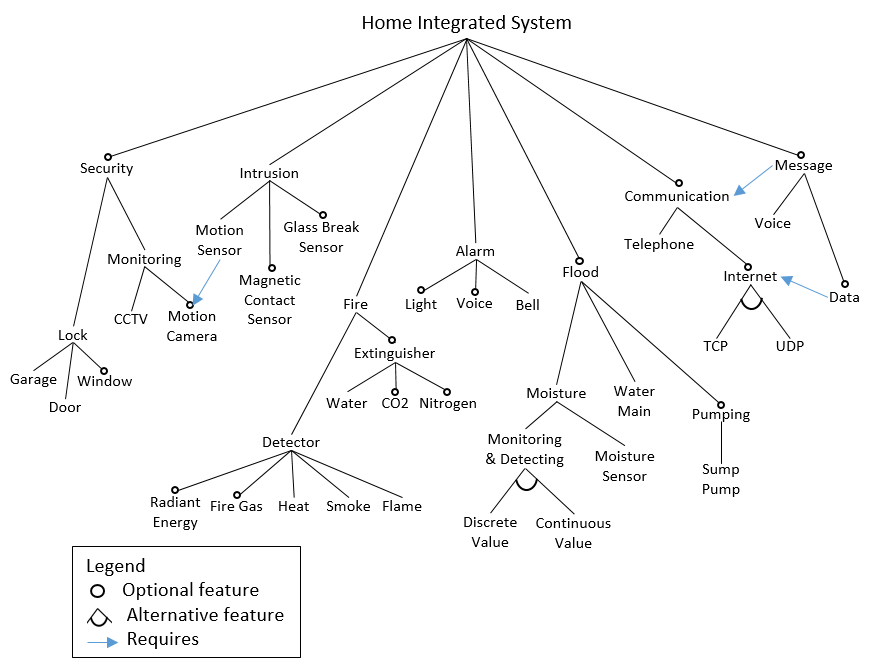
\includegraphics[width=1\textwidth]
		{pics/hisfd4.png}
	\caption{Home Integration System Feature Diagram}
	\label{fig:FD1}
\end{figure}
\vspace{-1cm}
\begin{center}
	{\small Source: \citep{paper.lee.featurebinding} (with additional changes)}
\end{center}

The figure above shows a set of features for Home Integrated System (HIS) \citep{paper.clarke.variability}. There are several features which can be chosen by users, such as {\it Fire, Flood, Alarm, Intrusion}, etc. Some features are general feature which consist of or implemented by the features followed. An {\it Alarm} feature consists of {\it Bell, Voice}, or {\it Light} feature. Then, an {\it Internet} feature implemented by {\it TCP} or {\it UDP} feature. 

A feature model is organized based on the visible characteristics of software \citep{paper.lee.featuremanagement}. It can be very large if the number of features available is also increasing. If a feature model has a large number of features, such as Linux kernel with more than 10.000 features \citep{book.apel.FeatureOrientedSoftware}, it can cause the selection of features process be more complex. To address this problem, the features in the feature model can be grouped based on their functions in general. By grouping the features, the complexity of the feature model can be reduced. Figure \ref{fig:FMGroup1} shows the example of grouped features represented using feature diagram.

\begin{figure}
	\centering
	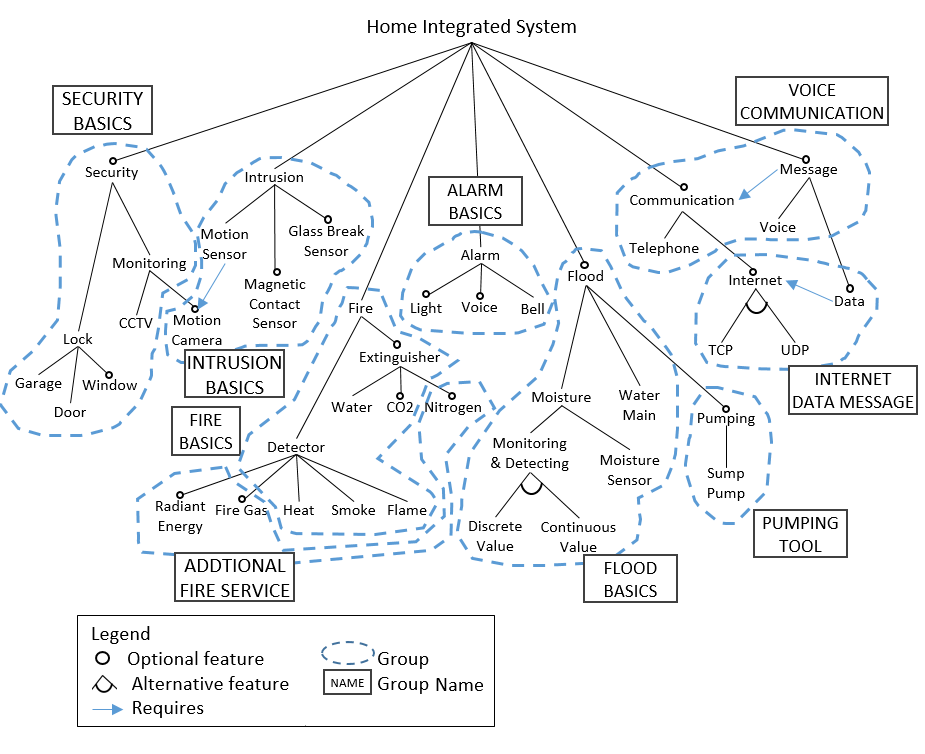
\includegraphics[width=1\textwidth]
	{pics/hisfd4group3.png}
	\caption{Home Integration System Feature Diagram with Grouping}
	\label{fig:FMGroup1}
\end{figure}
\vspace{-1cm}
\begin{center}
	{\small Source: \citep{paper.lee.featurebinding} (with additional changes)}
\end{center}

There are several groups of basic features, as shown on the figure, such as {\it Security Basics, Intrusion Basics, Fire Basics, Flood Basics,} and {\it Alarm Basics}. Moreover, there are features grouped to be additional features, such as {\it Additional Fire Services, Voice Communication, Pumping Tool,} and {\it Internet Data Message}. The features grouped by the common services they provide and the relationship they have. Moreover, the features can be grouped not only by common services they provide, but also by their common domains (e.g. basic or special features for a module), by the target of the users (e.g. small or large companies), and so on.

By now, the selection of features to be included in a software product in ABS is done by listing the features chosen using product selection language (PSL) \citep{paper.hanle.ABStutorial}. It could make the selection of features difficult to do, even more for a user. Thus, the grouped features are intended for the users so they can choose the features easily. As they do not need to see and choose the features based on the feature diagram structure. Moreover, the grouped features need to be made concrete, i.e. visual representation of the grouped features. By using the visual representation of the grouped features, it is expected that the users could choose the features less complex.

In this research the feature grouping mechanism will be made and visualized. The visualization is done by using a simple web application as a tool support. The grouped features and its visualization are intended for users so they can make a selection of features easily. Moreover, the purpose of the feature grouping is to reduce the complexity while doing the features selection. Then, it is expected that the visualization could make the feature selection process more efficient.

Case studies will be used in this research. Those are Charity Organization System (COS) and Odoo Sales module. COS is a system developed to help charity organizations and relies on software product line (SPL) approach and uses ABS language. Odoo Sales module is a part of Odoo software. Odoo is an open-source \citep{web.Odoo.whatIsOdoo,web.Odoo.ERPComparison} enterprise management software \citep{web.Odoo.whatIsOdoo}. COS and Odoo Sales module have features which can be used as the case studies for this research.

%-----------------------------------------------------------------------------%
\section{Research Questions}
%-----------------------------------------------------------------------------%
Based on the research purpose, the research questions which will be answered by this research are as follows:
\begin{enumerate}
	\item {\it How to group the features?}
	Features from feature model or feature diagram need to be grouped. Then, some mechanisms to group the features need to be made.
	
	\item {\it Is the use feature grouping mechanisms to select features better than using the original feature diagram?}
	The feature grouping mechanisms need to be evaluated as those are proposed to make the feature selection process less complex.
	
	\item {\it How grouped feature improve the efficiency of building software?}
	ABS use product selection language as input for generating a software. The grouped feature is intended for the users to choose the features less complex, thus it need to make the process of building the software more efficient.
	
	\item {\it How to make a visualization of the feature grouping?}
	As said on the previous section, the grouped features need to be made concrete (not only abstraction). One to address that is by make a visual representation of those features.
	
	\item {\it How to make the grouping mechanisms and implement them from feature model in ABS tools?}
	Features from feature diagram need to be grouped using some mechanisms. Then, those mechanisms need to be implemented and took the ABS feature model as input.
\end{enumerate}

%-----------------------------------------------------------------------------%
\section{Research Goals}
%-----------------------------------------------------------------------------%
There are several research questions that have been stated. Based on the background of this research and those research questions, there are several goals which will be the target of this research. The research goals are as follows: 
\begin{enumerate}
	\item The feature grouping mechanisms are made to specify how the features should be grouped. 
	
	\item Then, the feature grouping mechanism from feature model in the ABS tools is implemented. Thus, it can generate the feature grouping result from the ABS feature model.The visualization of the result of feature grouping mechanism also need to be implemented. This visualization is expected could be a way to improve the efficiency of building software from the grouped features.
	
	\item Then, the feature grouping mechanisms are evaluated as the result of the research question given.
\end{enumerate}

%-----------------------------------------------------------------------------%
\section{Benefits of Research}
%-----------------------------------------------------------------------------%
Many researchers are contributing in the development of ABS. This research will contribute in the development of ABS because this research goals are to provide the mechanism to group the features and visualize the result.

In practical term, the grouping of features, hopefully, can reduce the complexity while doing the features selection. The visualization of the features selection also gives ease for users to select the features. Then, as stated in the research goals, the visualization could be a way to improve the efficiency of building software from the grouped features.

%-----------------------------------------------------------------------------%
\section{Scope of Research}
%-----------------------------------------------------------------------------%
The aim of this research is to make a grouping mechanism for features and visualize them. To limit the topics discussed in this research, there are scopes of this research as follows:
\begin{enumerate}
	\item The focus of the work is to implement grouping mechanism and the visualization using web application. The grouping mechanism will be implemented in the ABS code generator (compiler back-end). Then, the visualization will be implemented in the web application.
	\item Analyze the grouping mechanism and the visualization using a case study. The case study used is Charity Organization System (COS) and Odoo sales module. The features are taken from COS and Odoo sales module features. For Odoo sales module, several features which are specific to the vendor will be ignored. It is because the ignored features could be not common features in a sales module of an enterprise management software.
\end{enumerate}

%-----------------------------------------------------------------------------%
\section{Outline}
%-----------------------------------------------------------------------------%
The outline of this thesis proposal is describe as follows:
\begin{itemize}
	\item Chapter 1 \babSatu \\
	Chapter 1 describes the introduction of the thesis proposal that includes the background, research questions, research goals and scope, and the systematic of writing.
	\item Chapter 2 \babDua \\
	Chapter 2 contains the literature review and theories which used in this research as the basis to support. This chapter explains software product lines, Abstract Behavioral Specification (ABS), and related works about feature grouping. Additionally, a brief explanation about enterprise software.
	\item Chapter 3 \babTiga \\
	Chapter 3 discuss about the research methodology which consists steps needed to do this research.
	\item Chapter 4 \babEmpat \\
	Chapter 4 explains about the case studies used in this research which are Charity Organization System and Odoo sales module features.
	%\item Chapter 5 \babLima \\
	%\item Chapter 6 \babEnam \\
	%\item Bab 7 \babTujuh \\%
\end{itemize}
	%-----------------------------------------------------------------------------%
\chapter{\babDua}
%-----------------------------------------------------------------------------%
This chapter contains the literature reviews which used as the basis of this research. The Software Product Lines, Abstract Behavioral Specification, and related work about feature grouping are explained in this chapter. Additionally, a brief explanation about enterprise software included in this chapter as it will be used as the case study for this research.

%-----------------------------------------------------------------------------%
\section{Software Product Lines}
%-----------------------------------------------------------------------------%
Common software development is focused in developing individual software one at a time to individual users (or market segment). The process starts with analyzing the user's needs, then doing the design, implementation, testing, and last deployment of the software. It could take more efforts and times to build software for individual users. One concept to address this challenge is Software Product Lines. It aims to reduce effort and time of development of each software for individual users in a similar domain \citep{book.apel.FeatureOrientedSoftware}.

The concept of Software Product Lines (SPL) is to build softwares from reusable software components instead of from scratch so that software development can be done more efficiently \citep{book.apel.FeatureOrientedSoftware}. By using the components which already prepared before, the software will be built according to the needs of each user. The softwares produced can be similar in one domain, but they are actually different because they are tailored for the specific needs of users \citep{paper.kastnerApel.FeatureOrientedSoftwareDevelopment}.

There are several promised benefits by using SPL concept \citep{book.apel.FeatureOrientedSoftware,paper.kastnerApel.FeatureOrientedSoftwareDevelopment,book.pohl2005.softwareProductLineEngineering}. First, the software could be produced faster because the development process which uses reusable components. Second, it can reduce the effort and cost because the reusable components have already done before and the users don't need to pay for the cost of design and development software from scratch. Then, it can improve quality because the reusable components can be checked and tested either in isolation or in many softwares. Last, the softwares produced could be tailored for specific needs of users.

%-----------------------------------------------------------------------------%
\subsection{Features}\label{SecFeatures}
%-----------------------------------------------------------------------------%
SPL uses feature-oriented approach in managing variability of the needs or requirements of users. In feature-oriented approach, the variability is represented by using features \citep{paper.kastnerApel.FeatureOrientedSoftwareDevelopment}. A feature is a software property that is used to capture commonalities or variabilities among software \citep{paper.czarnecki2005.mappingFeatureToModels}. For example, for {\it Chat} program, there are features such as {\it Text, Voice, Video Communication}, and so on.

The variability needs to be modeled in order to manage it. One approach to model the variability is using the feature model \citep{book.apel.FeatureOrientedSoftware,paper.kastnerApel.FeatureOrientedSoftwareDevelopment} and represented graphically by using feature diagram \citep{book.apel.FeatureOrientedSoftware}. The feature model will be discussed in section \ref{SecFM} and section \ref{SecFD}.

%-----------------------------------------------------------------------------%
\subsection{Feature Model}\label{SecFM}
%-----------------------------------------------------------------------------%
In SPL, one approach to express variability is by using feature model \citep{book.apel.FeatureOrientedSoftware}. According to \citep{paper.kastnerApel.FeatureOrientedSoftwareDevelopment}, a feature model is a model which describes the set of features and the relationships them. By using feature model, a valid choice of features can be shown \citep{book.apel.FeatureOrientedSoftware}. To represent the feature model in graphical notation, a standard representation is using feature diagram.

%-----------------------------------------------------------------------------%
\subsection{Feature Diagram}\label{SecFD}
%-----------------------------------------------------------------------------%
"A feature diagram is a graphical notation to specify a feature model"  \citep{book.apel.FeatureOrientedSoftware}. A feature diagram is a hierarchical representation like tree representation. In feature diagram, a node consists the feature name denotes a feature. Then, the root representing a concept (e.g., a software system) and its descendant nodes being features. The edges between the node describes their relationships, such as a node connected with empty bullet denotes an optional features and a node connected with filled bullet denotes a mandatory features. If a feature is mandatory, it must be selected whenever the parent feature is selected. Then, multiple a set of child features can be selected only one (alternative) or can be selected more than one (at least 1). The alternative features denoted by empty arch and the 'at least 1' features denoted by filled arch \citep{paper.kastnerApel.FeatureOrientedSoftwareDevelopment}. An example of feature diagram is shown in Figure \ref{fig:ExampleFD}.

\begin{figure}
	\centering
	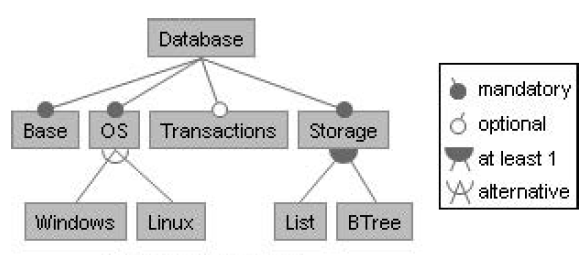
\includegraphics[width=0.6\textwidth]
	{pics/ExampleFD.png}
	\caption{Feature Diagram Example of a Small Database Product Line}
	\label{fig:ExampleFD}
\end{figure}
\vspace{-1cm}
\begin{center}
	{\small Source: \citep{paper.kastnerApel.FeatureOrientedSoftwareDevelopment}}
\end{center}

%-----------------------------------------------------------------------------%
%-----------------------------------------------------------------------------%
%-----------------------------------------------------------------------------%
\section{Abstract Behavioral Specification}
%-----------------------------------------------------------------------------%
Abstract Behavioral Specification (ABS) is a language which developed for high variability and configurable software such as software product lines (SPL) \citep{paper.clarke.variability,paper.hanle.ABStutorial}. As said in \citep{paper.clarke.variability}, "ABS is designed to fill the niche between design-oriented formalisms such as UML and feature description language FDL, on one hand, and implementation-oriented formalisms such as Spec\# and JML, on the other hand". So ABS is a modeling language but it can be executed and generated to other languages such as Java, Maude, or Scala \citep{paper.hanle.ABStutorial}.

ABS was developed by researchers in HATS (Highly Adaptable and Trustworthy Software using Formal Models) project \citep{thesis.niken.deltaRelationalMappingUsingABS} and equipped with ABS tool suite \citep{paper.wong.abstools}. ABS tool suite consists several tools which assist modeling in ABS such as compiler front-end, code generator, ABS plugin, etc. ABS front-end compiler used for code checking and translation code into an internal representation. Then the code generator, use the internal representation and generate it into other languages like Java, Scala, and Maude. To provide editing, visualizing, type checking, and executing, ABS can be integrated with Eclipse IDE which extended by ABS plugin \citep{paper.wong.abstools}.

The architecture of ABS is separated into two groups of layers, namely Core ABS and Full ABS \cite{paper.hanle.ABStutorial}. Core ABS consists several layers which provides modern programming languages like Java or Scala, concurrency, synchronization, standard contracts, and behavioral interface. Above the layers of Core ABS, there are extensions which provide product line engineering, deployment components, and runtime components. These extensions layer called the Full ABS. The architecture of ABS shown in Figure \ref{fig:ArchitectureOfABS}.

\begin{figure}
	\centering
	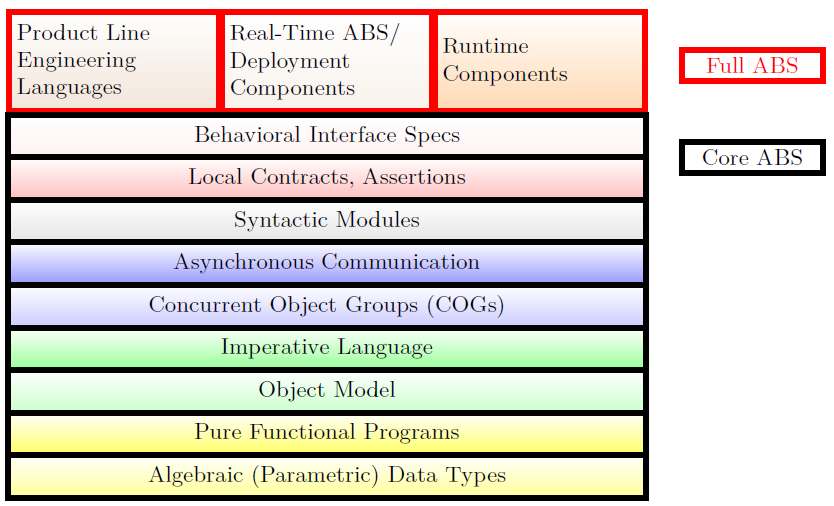
\includegraphics[width=0.8\textwidth]
		{pics/ArchitectureOfABS.png}
	\caption{The Architecture of ABS Language}
	\label{fig:ArchitectureOfABS}
\end{figure}
\vspace{-1cm}
\begin{center}
	{\small Source: \citep{paper.hanle.ABStutorial}}
\end{center}

In section \ref{SPLABS}, product line engineering in ABS is explained more. Then the ABS Compiler, as a part of the ABS tool suite, is explained in section \ref{ABSCompiler}.

%-----------------------------------------------------------------------------%
\subsection{Software Product Line in ABS}\label{SPLABS}
%-----------------------------------------------------------------------------%
SPL is an extension from the Core ABS. There are four special languages to represent product line in ABS \citep{paper.clarke.variability,paper.hanle.ABStutorial}, which are:
\begin{itemize}
	\item Micro Textual Variability Language ($\mu$TVL).
	This language is used to express the variability using feature models. The discussion about feature models in ABS is in section \ref{FeatureModelABS}.
	
	\item Delta Modeling Language (DML).
	This language is used to express the code-level variability of ABS. Delta used to specify transformation of the core ABS code, such as additions, removals, or modifications some methods or attributes. Delta modeling discussed more in section \ref{DeltaModeling}.
	
	\item Product Line Configuration Language (CL).
	This language is used to define the relationships between the feature model and the deltas. Product line configuration discussed more in section \ref{ProductLineConf}.
	
	\item Product Selection Language (PSL).
	This language is used to represent the softwares which can be generated. By define the selected features, a software can be generated. Product selection language discussed more in section \ref{ProductSelection}.
\end{itemize}

The relationship between these languages is shown in Figure \ref{fig:RelationshipFourLanguages}.

\begin{figure}
	\centering
	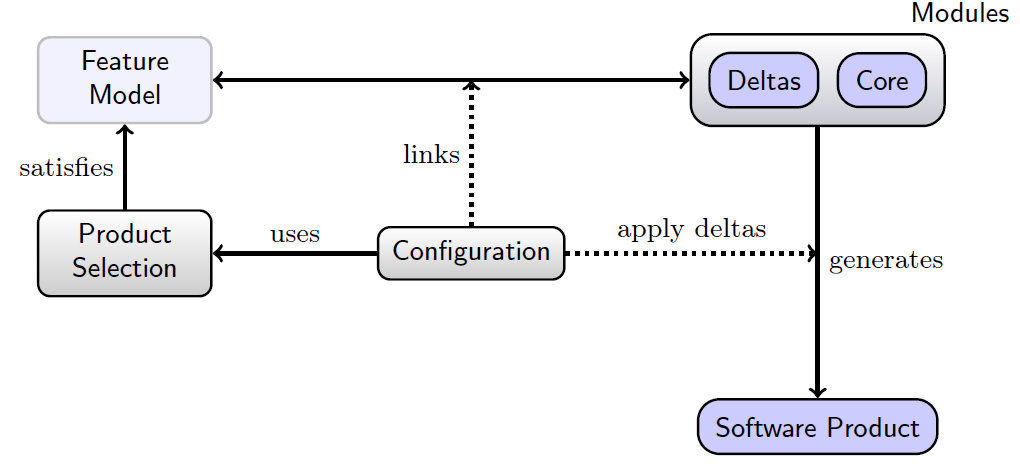
\includegraphics[width=0.7\textwidth]
	{pics/RelationshipFourLanguages.png}
	\caption{Relationship Between the Four Languages}
	\label{fig:RelationshipFourLanguages}
\end{figure}
\vspace{-1cm}
\begin{center}
	{\small Source: \citep{paper.clarke.variability}}
\end{center}


\subsubsection{Feature Models in ABS}\label{FeatureModelABS}
ABS has its feature model. All features will be declared in the feature model.
Johnsen \citep{paper.johnsen2014.deploymentVariabilityinDeltaOriented} gives the definition of feature model in ABS below.

\begin{quote}
	A feature model in ABS is represented textually as a forest of nested features where each tree structures the hierarchical dependencies between related features, and each feature in a tree may have a collection of Boolean or integer attributes. The ABS feature model can also express other cross-tree dependencies, such as mandatory and optional sub-features, and mutually exclusive features.
\end{quote}

The feature modeling language in ABS is using micro textual variability language ($\mu$TVL). $\mu$TVL is an extended subset of textual variability language (TVL). The design of $\mu$TVL is simpler than TVL in order to capture the essential feature modeling requirements \citep{paper.clarke.variability,paper.hanle.ABStutorial}. Beside that, it chosen because $\mu$TVL has formal semantics \citep{thesis.niken.deltaRelationalMappingUsingABS}.

$\mu$TVL has a grammar that shown in Figure \ref{fig:grammarFM}. For each feature, there is an identifier (which is name), an optional group of sub features, optional attributes, and optional constraints \citep{paper.clarke.variability,paper.hanle.ABStutorial}. Based on the grammar, FID denotes a name of a feature and then AID denotes a name of an attribute. Each sub feature has a group cardinality:
\begin{itemize}
	\item {\bf allof}. Indicates that all of the features can be chosen.
	\item {\bf oneof}. Indicates that just one of the features can be chosen (alternative).
	\item $n_{1}$ .. *. Indicates that the number of features can be chosen is from $n_{1}$ to all.
	\item $n_{1}$ .. $n_{2}$. Indicates that the number of features can be chosen is from $n_{1}$ to $n_{2}$.
\end{itemize}

\begin{figure}
	\centering
	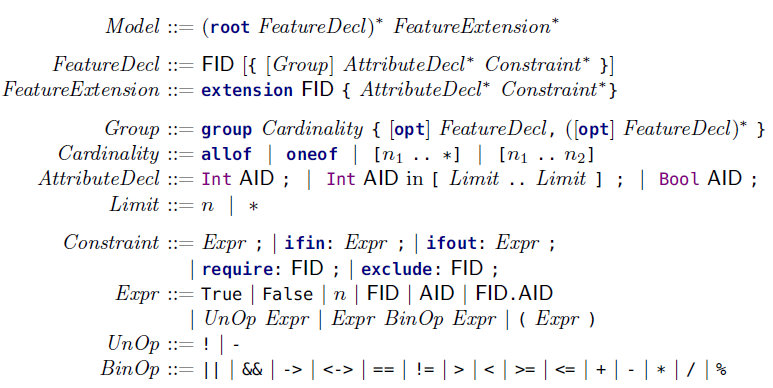
\includegraphics[width=0.9\textwidth]
	{pics/grammarFM.png}
	\caption{Grammar of $\mu$TVL}
	\label{fig:grammarFM}
\end{figure}
\vspace{-1cm}
\begin{center}
	{\small Source: \citep{paper.clarke.variability}}
\end{center}

The {\it AttributeDelc} clause specifies the declaration of attributes of a feature which can be an integer and boolean. An attribute or a feature could have constraints. That constraints is specified by the {\it Constraint} clause. There are several restrictions in the {\it Constraint} clause:
\begin{itemize}
	\item {\bf ifin:} {\it constraint}. Specifies that the {\it constraint} will be applied if the current feature {\bf is} selected.
	\item {\bf ifout:} {\it constraint}.  Specifies that the {\it constraint} will be applied if the current feature {\bf is not} selected.
	\item {\bf require:} FID. Specifies that the current feature needs the presence of other feature (which specifies with FID).
	\item {\bf exclude:} FID. Specifies that the current feature cannot be chosen if the other feature (which specifies with FID) is chosen, and vice versa.
\end{itemize}

An example of feature model in ABS is shown in Listing \ref{codeFMAccount}. The example shows the code of feature model for {\it Account} features. There are six features, group of sub features, constraints and attributes for the features. It also shows the features that optional (denotes with {\bf opt}) and mandatory (denotes without {\bf opt}).

\lstinputlisting[
	label={codeFMAccount},
	caption={Exampe Account Feature Model in ABS \citep{paper.hanle.ABStutorial}},
	firstline=1,
	style=ABS]{src/AccountFeatureModel.abs}

\subsubsection{Delta Modeling}\label{DeltaModeling}
Delta modeling uses the delta-oriented programming approach. Delta-oriented programming is an approach in SPL as an alternatives to feature-oriented programming approach \citep{paper.clarke.variability}. In delta-oriented programming, the aim is to provide a technique in generating software which modular and flexible in SPL \citep{paper.clarke.variability,paper.johnsen2014.deploymentVariabilityinDeltaOriented,paper.schulze2013.refactoringDeltaOrientedSPL}. Delta-oriented programming uses \textit{delta modules (deltas)} which the modules are associated with program modifications (add, remove, or modify code) \citep{paper.clarke.variability}. It's different from feature-oriented programming  which uses feature modules \citep{paper.kastnerApel.FeatureOrientedSoftwareDevelopment} that associated with each features \citep{paper.clarke.variability,paper.schulze2013.refactoringDeltaOrientedSPL}.

The implication of not associating delta module directly with features, it can obtain the flexibility, better code reuse, and get the ability to resolve conflicts when applying other delta modules \citep{paper.clarke.variability}. Other benefit of deltas is the abilities of delta module. A delta module can add, remove, and modify code. 

\begin{figure}
	\centering
	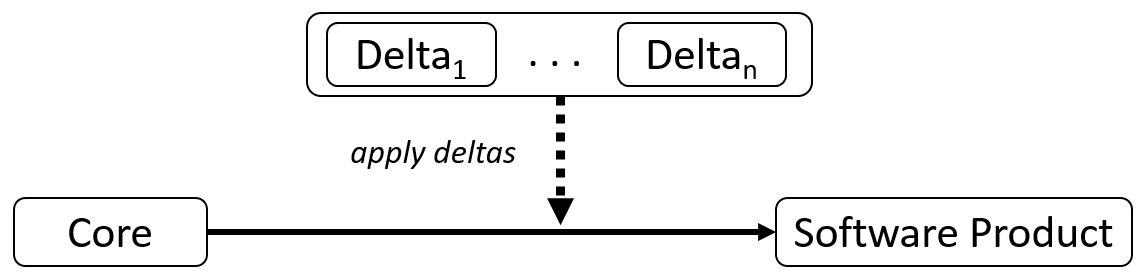
\includegraphics[width=0.9\textwidth]
	{pics/applicationOfDelta2.png}
	\caption{The Application of Delta Modules}
	\label{fig:applicationOfDelta}
\end{figure}
\vspace{-1cm}
\begin{center}
	{\small Source: \citep{paper.hanle.ABStutorial}}
\end{center}

There are two divisions of implementation of SPL in delta-oriented programming \citep{paper.clarke.variability,paper.johnsen2014.deploymentVariabilityinDeltaOriented}. They are core modules and delta modules. The core modules consist classes which implement a complete software for the SPL. Then, to obtain a new variant of software, the delta modules are used to describe how to modify the core modules. The application of delta modules to get a new software variant is shown in Figure \ref{fig:applicationOfDelta}.

\subsubsection{Product Line Configuration}\label{ProductLineConf}
Product line configuration (CL) uses to link the features in feature model with the delta modules so it can provide a complete specification for the product line \citep{paper.clarke.variability,paper.hanle.ABStutorial,paper.johnsen2014.deploymentVariabilityinDeltaOriented}. The declarations of which deltas applied to which features are written in here. Thus, it can make the process of analyzing the whole product lines more efficient \citep{paper.hanle.ABStutorial}.

Product line configuration consists set of features and set of delta modules. The connection between feature model, delta module, and the product line configuration is shown in Figure \ref{fig:connectionFmodDmodCL}. There are three configurations that could be specified in CL \citep{paper.hanle.ABStutorial,paper.johnsen2014.deploymentVariabilityinDeltaOriented}:
\begin{itemize}
	\item \textit{application condition} \\
	The \textit{application condition}, which denoted by \code[style=abs]{when} clause, associates the delta modules with the features. It describes that if the feature is selected, then use this delta(s) to implement the product line.
	
	\item \textit{parameters} \\
	The \textit{parameters} are derived from the feature attribute values which will be passed to the delta module.
	
	\item \textit{order of delta application} \\
	The \textit{order of delta application}, which denoted by \code[style=abs]{after} clause, is used to ensure the application of deltas is well-defined and resolve conflicts which could be occurred.
\end{itemize}

\begin{figure}
	\centering
	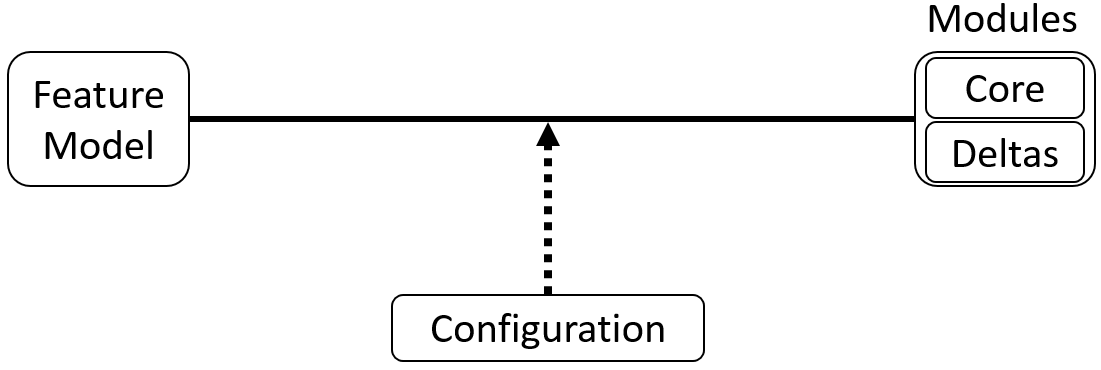
\includegraphics[width=0.7\textwidth]
	{pics/connectionFmodDmodCL2.png}
	\caption{The Connection Between Feature Model, Deltas, and CL}
	\label{fig:connectionFmodDmodCL}
\end{figure}
\vspace{-1cm}
\begin{center}
	{\small Source: \citep{paper.hanle.ABStutorial}}
\end{center}

An example of product line configuration shown in Listing \ref{codeAccountPL}. It is a configuration for the {\it Accounts} product line (which the features are shown in section \ref{FeatureModelABS}).

\lstinputlisting[
	label={codeAccountPL},
	caption={Account Product Line Configuration \citep{paper.hanle.ABStutorial}},
	firstline=1,
	style=ABS]{src/AccountPL.abs}


\subsubsection{Product Selection Language}\label{ProductSelection}
To specify the products (softwares) that could be generated, ABS uses the product selection language (PSL). Product selection language describes the features which will be included in the product and gives values to the attributes if needed \citep{paper.clarke.variability,paper.hanle.ABStutorial,paper.johnsen2014.deploymentVariabilityinDeltaOriented}. The syntax of PSL is pretty simple. To specify a product, the elements needed are the product name, the features used in that product, and values of attributes, if needed, to the features.

The example of product selection language is shown in Listing \ref{codeAccountProducts}. There are examples of products of {\it Accounts} product line. For example, \textit{CheckingAccount} product is built from \textit{Type} feature and \textit{Check} feature.

\lstinputlisting[
	label={codeAccountProducts},
	caption={PSL of Account Product Line \citep{paper.hanle.ABStutorial}},
	firstline=1,
	style=ABS]{src/AccountProducts.abs}


%-----------------------------------------------------------------------------%
\subsection{ABS Compiler}\label{ABSCompiler}
%-----------------------------------------------------------------------------%
ABS has a tool suite that used as a platform for developing and analyzing the ABS code \citep{paper.wong.abstools}. In ABS tool suite, there are two tools that used to be a compiler. They are compiler front-end and compiler back-end. The process to compile the ABS code and generate it to be a other language is shown in Figure \ref{fig:ABScompilerFlow}. ABS compiler front-end is used to translate the ABS code into an internal representation, then the ABS compiler back-end will use the internal representation to generate other languages.

\begin{figure}
	\centering
	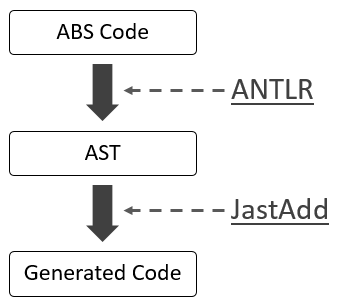
\includegraphics[width=0.5\textwidth]
	{pics/ABScompilerFlow.png}
	\caption{ABS Compiler Process Flow}
	\label{fig:ABScompilerFlow}
\end{figure}

In section \ref{ABSFrontEnd}, ABS compiler front-end is explained more. Then, the explanation of ABS compiler back-end is in section \ref{ABSBackEnd}.  

%-----------------------------------------------------------------------------%
\subsubsection{ABS Compiler Front-End}\label{ABSFrontEnd}
%-----------------------------------------------------------------------------%
ABS compiler front-end is used to translate the ABS code into an internal representation \citep{paper.wong.abstools}. The internal representation later will be used to check the ABS code for syntax and semantic errors. The compiler front-end takes ABS codes, such as core, feature model, delta modules, configuration, and product selection as inputs and translates them into the internal representation. From the internal representation of feature model, a valid combination of features can be found and used to validate the product selections.

The internal representation is called the Abstract Syntax Tree (AST) \citep{thesis.niken.deltaRelationalMappingUsingABS,paper.wong.abstools}. AST is a representation of the language constructions and formed as a tree \citep{paper.hedin.jastadd}. To translate ABS code into AST, the ABS compiler front-end uses a tool called ANTLR. ANTLR is a parser generator which can be used to read, process, execute, or translate structured text or binary files \citep{web.ANTLR.aboutANTRLParser}. ANTLR also can build the AST by providing grammar annotations. The grammar annotations used to indicate what tokens are treated as subtree roots, leaves, or to be ignored with respect to tree construction. To construct a tree with special structure, the ANTLR must be provided with the tree definitions \citep{web.ANTLR.ANTRLTreeConstruction}. In ABS, it's located in the abstract grammar which specified in \code{.ast} file.

The abstract grammar is defined in an \code{.ast} file called \code{ABS.ast}. A partial representation of ABS class hierarchy defined in \code{ABS.ast} is shown in Figure \ref{fig:ABSastHierarchy}.

\begin{figure}
	\centering
	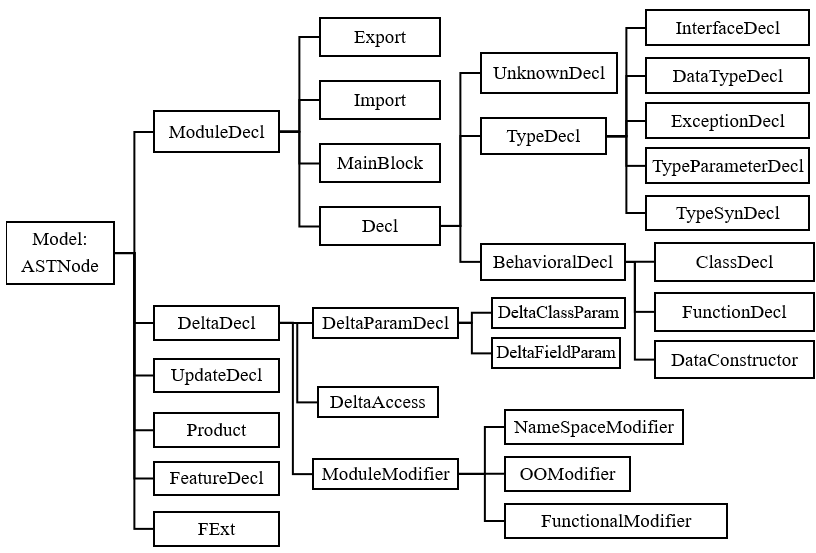
\includegraphics[width=0.8\textwidth]
	{pics/ABSastHierarchy.png}
	\caption{ABS.ast Hierarchy Represented in Diagram}
	\label{fig:ABSastHierarchy}
\end{figure}

%-----------------------------------------------------------------------------%
\subsubsection{ABS Compiler Back-End}\label{ABSBackEnd}
%-----------------------------------------------------------------------------%
The ABS compiler front-end has translated the ABS code into AST, then ABS compiler back-end uses the AST as an input to generate it into other languages. It can generate code to either executable programs in implementation languages, such as Java or Scala, or rewriting systems for simulation and analysis, such as Maude \citep{paper.wong.abstools}. To generate the AST to other languages, ABS uses JastAdd\footnote{http://jastadd.org/web/documentation/concept-overview.php} as the tool.

JastAdd is a meta-compilation system which designed to support extensible implementation of compilers and related tools like analyzers or transformation tools \citep{web.JastAdd.JastAddOverview}. By using JastAdd, the compiler can be extended by adding module that contain new abstract syntax and computations on the AST. The abstract syntax is modeled as a class hierarchy. It's modeled from the corresponding code which generated. 

JastAdd supports a capability for implementing behavior in the form of attributes \citep{web.JastAdd.JastAddOverview}. Attributes are attached to the AST nodes in AST and the values could be integers, composite values like set, or reference values which are stated using equations. Moreover, the values could point to other nodes in AST or access other attributes \citep{thesis.niken.deltaRelationalMappingUsingABS}.

The classes in the hierarchy called AST classes because they model nodes in the AST \citep{web.JastAdd.JastAddOverview}. There are method API formed to the classes which correspond to each attributes. By using the API, a programmer can get the correct value of the attribute according to the equation \citep{thesis.niken.deltaRelationalMappingUsingABS}.

ABS compiler back-end uses the \textit{aspects} of JastAdd to do the code generation. According to \citep{web.JastAdd.JastAddReferenceManual}, JastAdd will read the aspects files and weaves the aspect declarations into the appropriate AST classes. By adding a \code{.jadd} file, the AST classes could be added some ordinary fields and methods \citep{web.JastAdd.JastAddReferenceManual}. Therefore, a behavior could be added to the AST classes such as pretty printing behavior.


%-----------------------------------------------------------------------------%
%-----------------------------------------------------------------------------%
%-----------------------------------------------------------------------------%
\section{Feature Grouping and Related Works}
%-----------------------------------------------------------------------------%
In ABS, a set of features is defined in feature model. Then, the selection of features that will be included in a software is done by writing the features using product selection language (section \ref{ProductSelection}). The feature model can consist a feature tree in implementation level. For example, from Figure \ref{fig:FD1} which shown the example of Home Integrated System feature diagram, a \textit{Heat} feature is a child of \textit{Detector} feature which a child of \textit{Fire} feature. The deep level could be vary based on the feature model.

The feature model also can be very large if the number of features available is increasing, such as Linux kernel with more than 10.000 features \citep{book.apel.FeatureOrientedSoftware}. The selection of features could be more difficult to do. Even more for users to choose the features they want. To address this problem, the features in the feature model can be grouped.

Previous researchers have done researches about how to group the features. Two of those are by using the feature binding unit (FBU) \citep{paper.lee.featurebinding,paper.lee.featuremanagement} and views \citep{paper.hubaux2013.supportingMultiplePerspective}.

%-----------------------------------------------------------------------------%
\subsection{Feature Binding Unit, Lee et al.}
%-----------------------------------------------------------------------------%
Lee et al \citep{paper.lee.featuremanagement} define the feature binding unit (FBU) as: "A set of features that are related to each other by the relationships in a feature model". Feature binding consists a set of features that run a common service an must exist together to perform a the correct service \citep{paper.lee.featurebinding,paper.lee.featuremanagement}. As said by Lee \citep{paper.lee.featuremanagement} that the grouping can reduce the complexity in managing the variations, thus it can reduce the complexity for users to choose the common services they want (even if the product selection language still use features to specify a software).

The examples of feature binding units are shown in Figure \ref{fig:FeatureModelFBU}. The FBU is a set of features denoted by blue-dotted-line circle. For example, there are several basic features, such as {\it Security Basics, Intrusion Basics, Fire Basics, Flood Basics,} and {\it Alarm Basics}. Then there are features grouped to be additional features, such as {\it Additional Fire Services, Voice Communication, Pumping Tool,} and {\it Internet Data Message}. The features are grouped by the common services they provided and the relationship they had in the feature model.

\begin{figure}
	\centering
	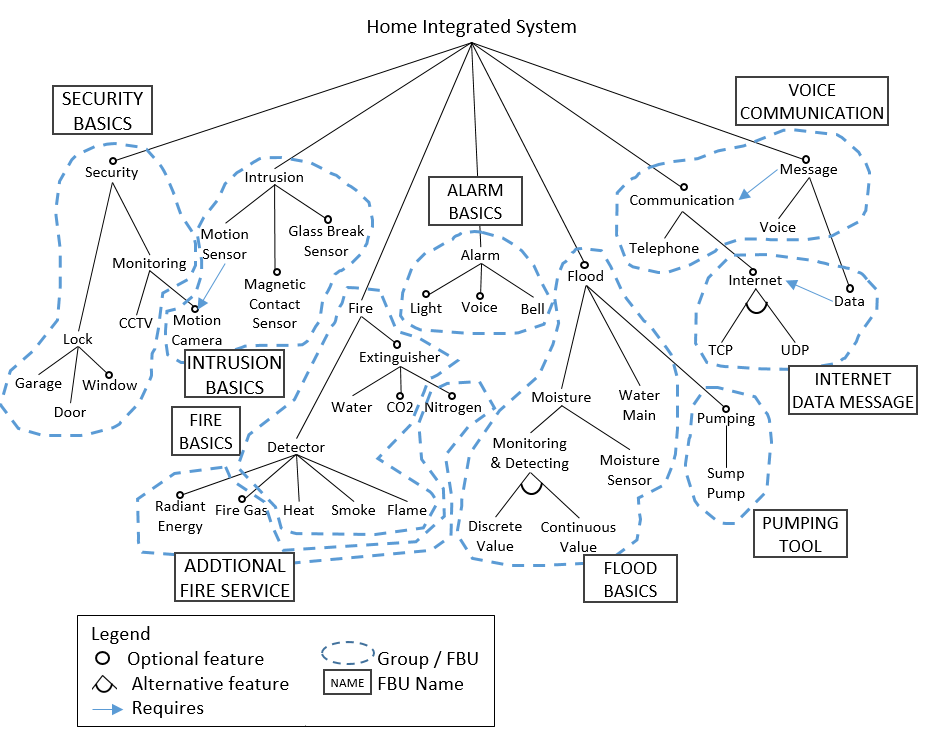
\includegraphics[width=0.8\textwidth]
	{pics/hisfd4group3a.png}
	\caption{Home Integration System Feature Diagram with Grouping}
	\label{fig:FeatureModelFBU}
\end{figure}
\vspace{-1cm}
\begin{center}
	{\small Source: \citep{paper.lee.featurebinding} (with additional changes)}
\end{center}

%-----------------------------------------------------------------------------%
\subsection{Views, Hubaux et al.}
%-----------------------------------------------------------------------------%
Hubaux et al \citep{paper.hubaux2013.supportingMultiplePerspective} said that there are two challenges that failed to address by feature selection process using the original feature model. Those are (1) configuring the feature selection environment according to the users' profile (e.g knowledge, role, preferences, etc) and (2) managing the complexity from the size of the feature diagram.

View is one to address those challenges. Hubaux et al \citep{paper.hubaux2013.supportingMultiplePerspective} define view as: "a simplified representation of a feature diagram that has been tailored to the stakeholders (users) profile or generalized to a particular combination of features". Using view, it facilitate the users to focus only on those parts that are relevant to them. Thus, it could reduce the complexity of choosing the features. 

There are three issues that Hubaux et al focus on. Those are as follow.
\begin{itemize}
	\item View Specification \\
	There are two ways to specify views. First, by enumerating the features that appear for each views. It can be done by tagging each feature with the names of the views they belong to. Second, by using a language that takes advantage of the feature diagram tree structure. They using XPath as the language that designed to navigate in tree-structures.
	
	\item View Coverage \\
	It is important to guarantee that a decision for each feature in feature diagram has been made (selected or not). One way is to fulfill the sufficient coverage condition. Sufficient coverage condition means that all features should appear in at least one view, hence no feature can be left undecided.
	
	\item View Visualization \\
	The views need to be made concrete by using visualization. Hubaux et al define the goal of a visualization are:
	\begin{itemize}
		\item showing only features that belong to a view, and 
		\item including features that are not in the view but that provide context and thereby allow the user to make informed decisions.
	\end{itemize}
\end{itemize}

%-----------------------------------------------------------------------------%
\subsection{Comparison}
%-----------------------------------------------------------------------------%
Previous researchers have attempted to manage the complexity of features selection by grouping the features. Lee et al introduce the feature binding unit (FBU) which each of it consists features that belong to the same service provided. Then Hubaux et al introduce view as a set of features that has been tailored to users profile. Both of them trying to group the features in different ways, but there is no grouping mechanism based on the features domains (e.g. basic or special features for a module), the target of the users (e.g. small or large companies), and so on. Lee et al discuss how to group the features only by their common service. Then Hubaux et al discuss how to group the features in technical terms by tagging each feature with the names of the views (groups) they belong to.


\section{Enterprise Management Software}
As this research uses a part (module) of an enterprise management software, also known as enterprise software or enterprise application software, here is an brief explanation about enterprise software. 

Enterprise software is a software which allows companies to integrate business processes by sharing information across business functions and employee hierarchies \citep{book.olson2010.enterpriseIS}. It can replace multiple independent systems which process data to support particular business functions or processes. A lot of data used in an enterprise software. Fowler in \citep{book.fowler2002.patternsEnterpriseApp} said that an enterprise softwares are about 1) the display, manipulation, and storage of large amounts of data and 2) the support or automation of business processes with that data.

There are several types of enterprise software. Enterprise Resource Planning (ERP), Customer Relationship Management (CRM), and Supply Chain Management (SCM) are examples of enterprise softwares \citep{web.erp.typeEnterpriseSystem}. They support companies to do some business processes more efficiently. For example, an ERP software used to integrate some business processes, such as sales, purchasing, finance, human resources, and inventory management, so it can communicate and share data among departments in a company. In a common way, each function of an enterprise software is called module. So that the function to support sales process is called sales module. Modules in an enterprise software can be different based on the types of the enterprise software.

In conclusion, enterprise softwares are intended to solve an enterprise-wide problem. It aims to improve the enterprise's productivity and efficiency by providing business support functionality. Then, several types of enterprise software are intended to help companies to run their business processes based on the type of the business process.
	%-----------------------------------------------------------------------------%
\chapter{\babTiga}
%-----------------------------------------------------------------------------%
Based on the research background, questions, goals, and scope that have been stated on the previous chapter, the research methodology which used in this research is as follows.

\begin{figure}
	\centering
	\includegraphics[width=1\textwidth]
	{pics/ResearchFlow2.png}
	\caption{Stages of Research}
	\label{fig:researchMethodFig}
\end{figure}

As shown in Figure \ref{fig:researchMethodFig}, there are 10 stages that must be done in this research. It begin with the literature review to get theories which can be used as basis of this research, such as definitions, related works, and so on. Then, the feature grouping mechanisms will be made. After that, the tools are implemented. There are two tools used in this research. First, tool for generating the feature grouping mechanisms from the feature model using ABS tools. Second, tool for visualizing the grouped feature. In another word, the tool is an user interface for the features selection. Then, the tools will be tested using case studies. There are two case studies used, Charity Organization System and Odoo Sales module. Then, the tools along with the grouping mechanisms will be analyzed. After that, the grouping mechanisms will be evaluated. Finally, the report of this research will be written along with the conclusion.

%-----------------------------------------------------------------------------%
\section{Literature Review}
%-----------------------------------------------------------------------------%
At this stage, a literature study will be conducted. The sources the literature study come from a wide range, such as books, scientific articles, papers, and web to get information and knowledge related which used as the supporting theory required to perform this research. The supporting knowledge needed are about the software product line (SPL), Abstract Behavioral Specification (ABS) and its SPL support, related works that have been conducted about grouping features, and enterprise management software.

%-----------------------------------------------------------------------------%
\section{Creating Feature Grouping Mechanism}
%-----------------------------------------------------------------------------%
At this stage, the feature grouping mechanisms will be made. The feature grouping mechanisms will be made using features on the case studies (Section \ref{casestudy}). The stage of creating feature grouping mechanisms conducted first because the result of this stage will be used as basis to implement the tools and evaluating the result.

%-----------------------------------------------------------------------------%
\section{Implement Tool for Grouping in ABS Tools}
%-----------------------------------------------------------------------------%
After the feature grouping mechanisms are made, next stage is implementing tool for grouping in ABS tools. ABS tools have ABS compiler back-end (code generator) which using JastAdd as the tool to generate other languages. It can be used to implement the grouping mechanisms and generate another output.

%-----------------------------------------------------------------------------%
\section{Implement User Interface for Selecting Feature}
%-----------------------------------------------------------------------------%
The next stage is implementing the user interface for selecting features (in ABS term, product selection). As stated in previous section that the grouping mechanisms should be made concrete. By using web application, the features that have been grouped can be shown. The inputs are features that have been grouped from the previous stage.

%-----------------------------------------------------------------------------%
\section{Test the Tools Using Case Studies}
%-----------------------------------------------------------------------------%
Tools then will be tested using case studies. There are two case studies used in this research, Charity Organization System and Odoo Sales module (Section \ref{casestudy}). 

	%-----------------------------------------------------------------------------%
	\subsection{Test Using Charity Organization System}
	%-----------------------------------------------------------------------------%
	Charity Organization System (COS) will be used to see if the tools can group features using the grouping mechanisms, visualize them using the user interface, and conduct the product selection process. COS is used because it has been developed by researchers in RSE Lab in Faculty of Computer Science UI using SPL approach and ABS language.
	
	%-----------------------------------------------------------------------------%
	\subsection{Test Using Odoo Sales Module}
	%-----------------------------------------------------------------------------%
	To get a broader evaluation of the grouping mechanisms and the tools made, a test using Odoo Sales module will be conducted. Odoo Sales module has no ABS code implemented, but it has features which can be used to evaluate the grouping mechanisms and represent a part of an enterprise management system.

%-----------------------------------------------------------------------------%
\section{Analyze the Tools and the Outputs}
%-----------------------------------------------------------------------------%
Next stage is analyzing the outputs of the tools. The tools need to be analyzed to see if they can generate the grouped features which fit the grouping mechanisms and visualize the grouped features along with conducting the selection of features process (product selection).

%-----------------------------------------------------------------------------%
\section{Evaluate the Grouping Mechanism}
%-----------------------------------------------------------------------------%
After the tools have been made based on the grouping mechanisms and provide expected result, the next stage is evaluating the grouping mechanisms. Each grouping mechanism will be evaluated using several terms that related to grouping process, i.e. concerns of users, complexity of grouping, degree of specialization, and the abstraction principle. The evaluating process goal is not to find the best grouping mechanism, but it is to determine the advantages and disadvantages of each grouping mechanism using such terms.

%-----------------------------------------------------------------------------%
\section{Write Report and Conclusion}
%-----------------------------------------------------------------------------%
Finally, at this stage, the report of this research will be written along with the conclusion and the findings obtained during conducting this research.
	%-----------------------------------------------------------------------------%
\chapter{\babEmpat}\label{casestudy}
%-----------------------------------------------------------------------------%
There are two case studies used in this research, Charity Organization System and Odoo Sales module. This chapter discuss about those case studies.

%-----------------------------------------------------------------------------%
\section{Charity Organization System (COS)}
%-----------------------------------------------------------------------------%
Charity Organization System (COS)\footnote{http://rse.cs.ui.ac.id/?open=prices/charity} is a system developed to help charity organizations in addressing several issues, such as equal distribution of aid and monitoring process. The development of the system is a part of a project which conducted by researchers in RSE Lab in Faculty of Computer Science UI. There are several charity organizations which will be used this system. Their business processes could be have commonalities, but each charity organization could has different features needed in the system. To address that issue, COS is developed relies on software product line (SPL) approach and uses ABS language. Using SPL approach, each charity organization can choose features based on their need. Then, ABS is one language which relies on SPL approach. By using SPL and ABS, the process of developing each system for each charity organization could be done more efficient.

\begin{figure}
	\centering
	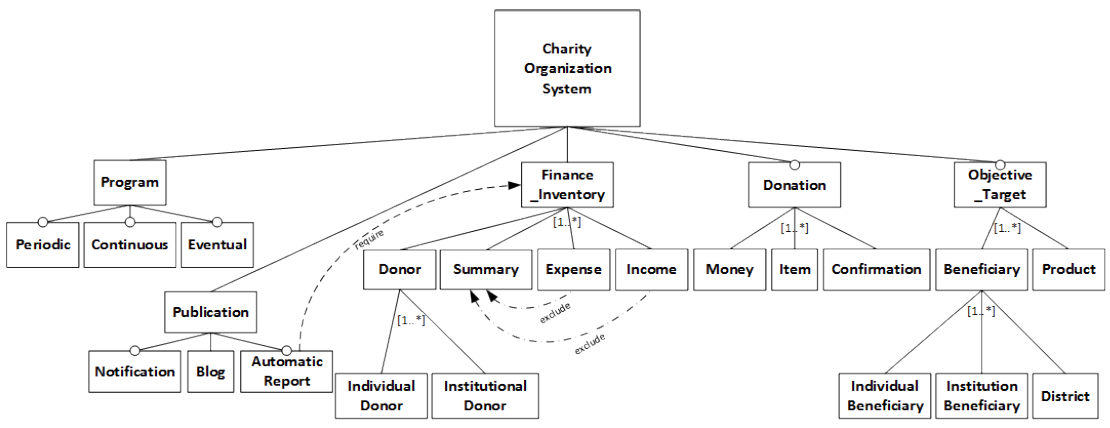
\includegraphics[width=1\textwidth]
	{pics/COSFD.png}
	\caption{Feature Diagram of Charity Organization System}
	\label{fig:COSFD}
\end{figure}

There are several features in COS\footnote{https://gitlab.com/IS4Charity/FeatureDiagram/tree/master/COS}. The feature diagram of COS shown in Figure \ref{fig:COSFD}. Then, the brief explanation of the features is as follow.

\begin{itemize}
	
	\item Program \\
	Types of events carried out by charity organizations.
	\begin{itemize}
		\item Periodic \\
		Event that made within a certain time frame.
		\item Continuous \\
		Event that made routinely.
		\item Eventual \\
		Event that made only one time.
	\end{itemize}
	
	\item Publication \\
	Types of reports used by the charity organizations.
	\begin{itemize}
		\item Notification \\
		An announcement about donations to donors.
		\item Blog \\
		A post about charity activities held.
		\item Automatic Report \\
		An information thath automatically generated from financial data.
	\end{itemize}
	
	\item Finance Inventory \\
	Types of financial records required.
	\begin{itemize}
		\item Donor
		\begin{itemize}
			\item Individual Donor \\
			Record is derived from individual persons.
			\item Institutional Donor \\
			Record is derived from institutions or organizations.
		\end{itemize}
		\item Summary \\
		Recapitulation of the financial report on charities.
		\item Expense \\
		Details of the financial report on expenditures charities.
		\item Income \\
		Details of the financial report on incomes charities.
	\end{itemize}
	
	\item Donation \\
	Types of contributions given in charity events.
	\begin{itemize}
		\item Money \\
		A cash form donation.
		\item Item \\
		A goods form donation.
		\item Confirmation \\
		An acceptance report of delivery donations that have been made.
	\end{itemize}
	
	\item Objective Target \\
	Types of programs aimed to individuals, institutions, or specific places.
	\begin{itemize}
		\item Beneficiary
		\begin{itemize}
			\item Individual Beneficiary
			Individual persons are the target of recipients.
			\item Institution Beneficiary \\
			Institutions or organizations are the target of recipients.
			\item District \\
			Specific area is the target of recipient.
		\end{itemize}
		\item Product
		Program that distributes goods.
	\end{itemize}
\end{itemize}


%-----------------------------------------------------------------------------%
\section{Odoo Sales Module}
%-----------------------------------------------------------------------------%
Odoo is an open-source \citep{web.Odoo.whatIsOdoo,web.Odoo.ERPComparison} enterprise management software \citep{web.Odoo.whatIsOdoo}. It is a suite consists several application modules, such as sales, accounting, manufacturing, purchasing, warehouse management, project management, etc. Odoo is targeting all sizes of companies (small, medium, and large companies). The goals of Odoo are to help the companies to manage, automate, measure and optimize their operations, finances and projects.

As said above, there are several modules in Odoo. One of it is Sales module\footnote{https://www.odoo.com/page/sales}. In Sales module, there are several features which help the users to do sales activity, such as creating quotation, taking sales order, and managing price-lists. Odoo Sales module has 28 features \citep{web.Odoo.OdooSalesFeatures}. The features are as follow.
\begin{itemize}
	\item Quotation Builder. \\
	Build quotation from the predefined products, price lists and templates.
	
	\item Quotation template \\
	Used to design quotation templates that can be reused.
	
	\item Upselling \\
	Quotations are optimized to help users sell more: propose extra options, apply closing triggers, discounts, etc.
	
	\item Electronic Signature \\
	Allow the customers to review and sign their quotations online.
	
	\item Contracts \\
	Record contracts and track invoicing phases, renewal and upselling.
	
	\item Sales Orders \\
	Convert quotation into sales order. Possibility to modify the sales order, remain opened, invoice kits. 
	
	\item Product Variants \\
	Create configurable products with multiple variants (size, color, etc.) and options.
	
	\item Product Types \\
	Manage services, physical products to delivery, electronic products and consumables.
	
	\item Manage invoicing from sales order \\
	Invoicing policy is configured in the product but managed from the sales order.
	
	\item Price-lists \\
	Price-list rules used to compute the right price based on customers conditions. 
	
	\item Dashboard \\
	Get a full overview on personal activities, next actions and performances.
	
	\item Recurring Contracts \\
	Manage subscriptions with Odoo's recurring contracts: billing, renewal alerts, extra options, MRR dashboard, etc.
	
	\item Reduce Data Entry \\
	Send quotes in just a few clicks, manage pipeline with drag and drop, etc.
	
	\item Time and Material Contracts \\
	Invoice customers based on time and materials with contracts.
	
	\item Customer Portal \\
	Customer can get an access to their quotes to track the status sales orders and delivery orders.
	
	\item Milestones \\
	Manage fixed price contract with invoicing based on milestones. Track invoices, forecast revenues and profitability.
	
	\item Discounts \\
	Apply discounts on every lines.
	
	\item Coupons \\
	Create names coupons or shared one to boost customer demands.
	
	\item Order and Invoicing Analysis \\
	Get statistics based on orders and \slash or invoices.
	
	\item Custom Alerts \\
	Follow key quotations and orders and get alerts based on relevant activities.
	
	\item Email Gateways \\
	All email communications automatically attached to the right order.
	
	\item On Boarding Emails \\
	Create template of emails for specific product to give information to buyers: access material, reminder of the service, etc.
	
	\item Multi company rules \\
	Automatically mirror sales orders and purchase orders in multi-company setup.
	
	\item SaaS KPIs \\
	Get a dashboard about all SaaS KPIs: Churn, MRR, Lifetime Value, CAC Ratio, upgrades / downgrades, etc.
	
	\item Modern User Interface \\
	A fast user interface designed for sales. 
	
	\item Mobile \\
	Sell on the road with Odoo's mobile user interface, working even if the users don't have an internet connection.
	
	\item Odoo eSign \\
	Use Odoo eSign to get signatures on NDAs, contracts or any PDF document.
	
	\item Incoterms \\
	Incoterms appear on the invoice.
\end{itemize}

%-----------------------------------------------------------------------------%
\section{Motivation for COS and Odoo Sales Modules Case Study}\label{MotivationCaseStudy}
%-----------------------------------------------------------------------------%
There are several reasons why Charity Organization System and Odoo Sales module chosen to be case study of this research. Those are as follow.

\begin{enumerate}
	\item Charity Organization System 
	\begin{enumerate}
		\item The case study is expected to give an overview concerning the problems in grouping features. This case study has features and  a feature model, but there is no grouping mechanism applied on it.
		\item The case study is addressed actual issues faced by the charity organizations. As stated, charity organizations are facing issues (equal distribution of aid and monitoring process). COS is developed as an intended to help those charity organization addressing the issues.
		\item The case study is developed using SPL approach and ABS language. As COS is developed using SPL approach and ABS language, so there is no need to re-create the system.
	\end{enumerate}
	\item Odoo Sales module
	\begin{enumerate}
		\item The case study is expected to give an overview concerning the problems in grouping features. This case study has features that have no grouping mechanism applied on it.
		\item The case study is expected to represent the scalability of enterprise management software features. An enterprise management software has many features in it. This case study is chosen to represent as a part of the enterprise management software.
		\item The case study is a well-known software with over 2 million users in over 120 countries \citep{web.Odoo.ERPComparison}.
	\end{enumerate}
\end{enumerate}
	%%%%%%%%-----------------------------------------------------------------------------%
\chapter{\babLima}
%-----------------------------------------------------------------------------%

%-----------------------------------------------------------------------------%
\section{Implementasi \f{Cluster}}
%-----------------------------------------------------------------------------%

%-----------------------------------------------------------------------------%
\subsection{Instalasi \f{Frontend}}
%-----------------------------------------------------------------------------%
Tabel model lain, ditunjukkan pada tabel \ref{tab:infohasti}. 
\begin{table}
	\centering
	\caption{Informasi \f{cluster} X}
	\newcolumntype{g}{>{\columncolor{headertbl}}c}
	\label{tab:infohasti}
	\begin{tabular}{|g|c|}
	\hline Host Name & X\\
	\hline Cluster Name & X\\
	\hline Certificate Organization & UI\\
	\hline Certificate Locality & Depok\\
	\hline Certificate State & West Java\\
	\hline Certificate Country & ID\\
	\hline Contact & X\\
	\hline URL & http://grid.ui.ac.id\\
	\hline
	\end{tabular}
\end{table}

Ada pagebreak disini.
%supaya rapih
\pagebreak

Another type of table
\begin{table}
	\centering
	\caption{Perbandingan Partisi \f{default} dan manual}
	\newcolumntype{g}{>{\columncolor{headertbl}}c}
	\label{tab:partdisk}
	\begin{tabular}{|g|c|c|}
	\rowcolor{headertbl}
	\hline & Partisi default & Partisi manual yang dilakukan\\
	\hline / & 16 GB & 30 GB\\
	\hline /var & 4 GB & 18 GB\\
	\hline swap & 1 GB & 2 GB\\
	\hline /export & 55 GB & 26 GB\\
	\hline
	\end{tabular}
\end{table}

Program menghasilkan keluaran seperti pada kode \ref{lst:raidready}. 

\begin{minipage}{\linewidth}
\begin{lstlisting}[caption={Keluaran output},label={lst:raidready}]
[root@nas-0-0 ~]# cat /proc/mdstat 
Personalities : [raid1] 
md0 : active raid1 sda4[0] sdb2[1]
      1917672312 blocks super 1.2 [2/2] [UU]
      
unused devices: <none>
[root@nas-0-0 ~]# mdadm --detail /dev/md0 
/dev/md0:
        Version : 1.2
  Creation Time : Fri May  3 15:38:52 2013
     Raid Level : raid1
     Array Size : 1917672312 (1828.83 GiB 1963.70 GB)
  Used Dev Size : 1917672312 (1828.83 GiB 1963.70 GB)
   Raid Devices : 2
  Total Devices : 2
    Persistence : Superblock is persistent

    Update Time : Tue May 28 11:27:49 2013
          State : clean 
 Active Devices : 2
Working Devices : 2
 Failed Devices : 0
  Spare Devices : 0

           Name : nas-0-0.local:0  (local to host nas-0-0.local)
           UUID : 0754726d:3dfbd4b9:42b0f587:68631556
         Events : 28

    Number   Major   Minor   RaidDevice State
       0       8        4        0      active sync   /dev/sda4
       1       8       18        1      active sync   /dev/sdb2
\end{lstlisting}
\end{minipage}

%-----------------------------------------------------------------------------%
\subsection{Konfigurasi}\label{cha:confcluster}
%-----------------------------------------------------------------------------%
Contoh verbatim dalam itemize : 
\begin{itemize}
\item \bo{Bold ini}\\
dijalankan perintah berikut : 
\begin{Verbatim}[frame=single]
# javac Ganteng.java
# java Ganteng
\end{Verbatim}
\paragraph{}
Perilaku sistem 
\begin{Verbatim}[frame=single]
# hai
# enable
# cd /export/rocks/install/
# create distro
# sh sesuatu.sh
# reboot
\end{Verbatim}
\paragraph{}

\item \bo{Menambahkan \f{package} pada \f{compute node}}\\
Langkah yang dilakukan adalah sebagai berikut : 
	\begin{enumerate}
	\item Masuk ke dalam direktori \co{/procfs/}
	\item Membuat/Mengubah berkas \co{xx.xml}. Jika tidak terdapat berkas tersebut, dapat disalin dari \co{skeleton.xml}.
	\item Menambahkan \f{package} yang ingin dipasang pada \f{compute node} diantara \f{tag} \co{<package>} seperti berikut : \co{<package>[package yang akan dipasang]</package>}.
	\item Menjalankan perintah berikut termasuk perintah untuk melakukan instalasi ulang seluruh \f{compute node}: 
	\begin{Verbatim}[frame=single]
# cd /export/somedir
# create
# run host
	\end{Verbatim}
	\end{enumerate}
	\paragraph{}
\end{itemize}
%-----------------------------------------------------------------------------%
\subsubsection{semakin ke dalam}
%-----------------------------------------------------------------------------%
\begin{minipage}{\linewidth}
\begin{lstlisting}[caption={Keluaran mentah untuk detail \f{job}}, label={lst:outqstatf},style=L]
[ardhi@xx ~]$ qstat -f 138
Job Id: 138.xx
    Job_Name = cur-1000-1np
    Job_Owner = ardhi@xx
    resources_used.cput = 27:21:35
    resources_used.mem = 86060kb
    resources_used.vmem = 170440kb
    resources_used.walltime = 27:24:50
    job_state = R
    queue = default
    server = hastinapura.grid.ui.ac.id
    Checkpoint = u
    ctime = Fri May 31 10:27:37 2013
    Error_Path = xx:/home/ardhi/xx/curcumin-1000/cur-1000-1np.e138
    exec_host = compute-0-5/0
    exec_port = 15003
    Hold_Types = n
    Join_Path = n
    Keep_Files = n
    Mail_Points = e
    Mail_Users = ardhi.putra@ui.ac.id
    mtime = Fri May 31 10:27:47 2013
    Output_Path = xx:/home/ardhi/xx/curcumin-1000/cur-1000-1np.o138
    Priority = 0
    qtime = Fri May 31 10:27:37 2013
    Rerunable = True
    Resource_List.nodes = 1:ppn=1
    session_id = 5768
    etime = Fri May 31 10:27:37 2013
    submit_args = cur-1000-1np.pbs
    start_time = Fri May 31 10:27:47 2013
    submit_host = xx
    init_work_dir = /home/ardhi/xx/curcumin-1000   
\end{lstlisting}
\end{minipage}

%-----------------------------------------------------------------------------%
\section{Pengujian} %lebih ke gimana cara ujinya
%-----------------------------------------------------------------------------%

%-----------------------------------------------------------------------------%
\subsection{Kasus Uji}
%-----------------------------------------------------------------------------%
Berwarna!
\begin{lstlisting}[caption=Potongan skrip submisi \f{job} melalui torqace,label={lst:grotorqace},style=shell]
# Go To working directory
cd $PBS_O_WORKDIR

#openMPI prerequisite
. /opt/torque/etc/openmpi-setup.sh

mpirun -np 5 -machinefile $PBS_NODEFILE mdrun -v -s \ 
	curcum400ps.tpr -o md_prod_curcum400_5np.trr -c lox_pr.gro
...
\end{lstlisting}
%-----------------------------------------------------------------------------%
\subsection{Kasus Uji}
%-----------------------------------------------------------------------------%
Contoh skrip yang dimasukkan pada \f{form} yang disediakan dapat dilihat pada kode \ref{lst:makebzip}.
\begin{lstlisting}[caption={Potongan \co{Makefile} \f{project}}, label={lst:makebzip},style=shell]
# Make file for MPI
SHELL=/bin/sh

# Compiler to use
# You may need to change CC to something like CC=mpiCC
# openmpi : mpiCC
# mpich2  : /opt/mpich2/gnu/bin/mpicxx
CC=mpiCC
...
...
\end{lstlisting}
	%%%%%%%%-----------------------------------------------------------------------------%
\chapter{\babEnam}
%-----------------------------------------------------------------------------%
Disini saya mencoba untuk menulis.

%-----------------------------------------------------------------------------%
\section{Hasil Pengujian}
%-----------------------------------------------------------------------------%
%-----------------------------------------------------------------------------%
\subsection{Hasil Pengujian Kasus Uji 1}
%-----------------------------------------------------------------------------%
Tabel lain. Hasil tersebut dapat dilihat pada tabel \ref{tab:hasilgrrd}.
\begin{table}
	\centering
	\caption{Hasil pengujian menggunakan gromacs}
	\label{tab:hasilgrrd}
	\begin{tabular}{|c|l|*{3}{c|}}
		\rowcolor{headertbl}
  		\hline % create horizontal line
  		No & \f{Timestep} & \multicolumn{3}{|>{\columncolor{headertbl}}c|}{Waktu eksekusi berdasar jumlah prosesor} \\
		\hhline{|>{\arrayrulecolor{headertbl}}*{2}{-}>{\arrayrulecolor{black}}*{3}{|-|}}
  		\rowcolor{headertbl} & & 1 & 2 & 5 \\
  		\hline 1 & 200ps & 20h:27m:16s & 12h:59m:04s & 5h:07m:03s \\
  		\hline 2 & 400ps & 1d:22h:40m:03s & 1d:02h:08m:47s & 10h:09m:39s \\
  		\hline 3 & 600ps & 2d:23h:29m:21s & 1d:14h:52m:52s & 15h:25m:22s \\
  		\hline 4 & 800ps & 4d:02h:05m:57s & 2d:03h:30m:07s & 20h:29m:38s \\
  		\hline 5 & 1000ps & 5d:03h:29m:12s & 2d:16h:32m:22s & 1d:01h:34m:38s \\
  		\hline
	\end{tabular}
\end{table}
%-----------------------------------------------------------------------------%
\section{Evaluasi Hasil Kasus Uji}
%-----------------------------------------------------------------------------%
%-----------------------------------------------------------------------------%
\subsection{Evaluasi Kasus Uji 1}
%-----------------------------------------------------------------------------%
Tabel \ref{tab:hasilgrrd} menunjukkan hasil uji coba pada penelitian ini.  Gambar \ref{fig:grafgro5} menunjukkan perbandingan waktu eksekusi pada aplikasi x dengan jumlah prosesor sebanyak 5 buah.

\begin{figure}
	\centering
	\includegraphics[width=1\textwidth]
		{pics/5np-gromacs-chart.pdf}
	\caption{Perbandingan waktu eksekusi x untuk 5 prosesor}
	\label{fig:grafgro5}
\end{figure}
\paragraph{}
	%%%%%%%%-----------------------------------------------------------------------------%
\chapter{\babTujuh}
%-----------------------------------------------------------------------------%
Pada bab terakhir ini, 
%---------------------------------------------------------------
\section{Kesimpulan}
%---------------------------------------------------------------

%---------------------------------------------------------------
\section{Saran}
%---------------------------------------------------------------

	
	%\printbibliography
	%
	% Daftar Pustaka
	%\include{pustaka}
	%
	\bibliography{bib}{}
	\bibliographystyle{abbrv}
	%\bibliography{references}{}
	%
	%\bibliographystyle{apalikerd}
	%\bibliographystyle{ieeetr} 
	
	%
	% Lampiran 
	%
	%%%%%%%\begin{appendix}
		%%%%%%%%
% @author  Andreas Febrian
% @version 1.00 
% 
% Hanya sebuah pembatas bertuliskan LAMPIRAN ditengah halaman. 
% 

\begin{titlepage}
	\centering 
	\vspace*{6cm}
	\noindent \Huge{LAMPIRAN}
	\addChapter{LAMPIRAN}
\end{titlepage}
		%%%%%%%\setcounter{page}{2}
		%%%%%%%%-----------------------------------------------------------------------------%
\addChapter{Lampiran 1 : Kode Sumber}
\chapter*{Lampiran 1 : Kode Sumber}
%-----------------------------------------------------------------------------%
\section*{\code{admin\_useraddmaster}} \label{cha:lampir-admin}
Skrip ini diletakkan pada direktori \co{/usr/sesuatu} dan hanya dapat dieksekusi oleh \f{root}. Skrip ini berguna untuk menambahkan pengguna baru sesuai dengan konfigurasi baru yang telah ditetapkan.
\begin{lstlisting}[style=L,caption={Skrip menambahkan pengguna baru},label={lst:adduser}]
#!/bin/csh -f
blah blah blah
blah blah blah
blah blah blah
blah blah blah
blah blah blah
\end{lstlisting}

\section*{\code{getuser.cron}} \label{cha:lampir-cronadmin}
Penjelasan skrip disini
\begin{lstlisting}[style=L,caption={\f{Cronjob} menambahkan pengguna baru},label={lst:cronadduser}]
#!/bin/bash
# Change these two lines to localize to your system:
# Adapted from /usr/local/sbin/admin_useradd

cat /dev/null > $userlist
for (( i=0; i<${#listemailto[@]}; i++ ))
do
        uname=${listusername[$i]}
        mailto=${listemailto[$i]}

        echo "User $uname created, please use torqace wisely." | mail -s "Torqace user registration" $mailto
done

\end{lstlisting}

%-----------------------------------------------------------------------------%
\addChapter{Lampiran 2 : Berkas Konfigurasi}
\chapter*{Lampiran 2 : Berkas Konfigurasi}
%-----------------------------------------------------------------------------%
\section*{compute.xml}
\begin{lstlisting}[caption={Berkas \co{compute.xml}},label={lst:excomp},language=XML]
<?xml version="1.0" standalone="no"?>
<kickstart>
<description>
	Compute node XML file
</description>
</kickstart> 
\end{lstlisting}

%-----------------------------------------------------------------------------%
\addChapter{Lampiran 8 : UAT dan Kuesioner}
%-----------------------------------------------------------------------------%
\begin{landscape}
\chapter*{Lampiran 8 : UAT dan Kuesioner}
\begin{longtable}{|c|p{7cm}|p{2.5cm}|p{3.5cm}|p{3.3cm}|p{1.8cm}|}
\caption{Tabel UAT dan Kuesioner} \label{tab:uattbl}\\
\hline
No. & \multicolumn{1}{c|}{Langkah Penggunaan} & Fitur Berjalan & Tingkat Kemudahan (1-5) & Tingkat Kepuasan (1-5) & Saran / Komentar \\ 
\cline{3-5} & & Berhasil /Tidak & 1:Sangat sulit ; \hspace{100pt} 5:sangat mudah & 1 : Sangat kecewa ; 5 : sangat puas &  \\ \hline
\multicolumn{ 6}{|>{\columncolor{headertbl}}c|}{Use Case : Login} \\ \hline
1.1 & Pengguna berada pada halaman depan torqace &  &  &  &  \\ \hline
1.2 & Pengguna memasukkan username dan password pada field yang telah disediakan.Kemudian menekan tombol 'login' &  &  &  &  \\ \hline
1.3 & Apabila Sukses, maka pengguna masuk ke dalam sistem dan dihadapkan pada menu utama &  &  &  &  \\ \hline
\multicolumn{ 6}{|>{\columncolor{headertbl}}c|}{Use Case : Register} \\ \hline
2.1 & Pengguna berada pada halaman registrasi pengguna torqace &  &  &  &  \\ \hline
2.2 & Pengguna memasukkan username,password, dan email pada field yang telah disediakan. Kemudian menekan tombol 'submit' &  &  &  &  \\ \hline
2.3 & Sistem akan mengonfirmasi masukan, dan akan mengirimkan email untuk memberitahu pengguna apabila proses pendaftaran telah selesai &  &  &  &  \\ \hline
\multicolumn{ 6}{|>{\columncolor{headertbl}}c|}{Use Case : Logout} \\ \hline
3.1 & Pengguna memilih menu untuk melakukan logout &  &  &  &  \\ \hline
3.2 & Sistem akan mengeluarkan pengguna, dan pengguna tidak dapat menggunakan fitur-fitur utama aplikasi &  &  &  &  \\ \hline
\multicolumn{ 6}{|>{\columncolor{headertbl}}c|}{Use Case : Upload Job Sederhana} \\ \hline
4.1 & Pengguna memilih menu upload file/project pada menu utama &  &  &  &  \\ \hline
4.2 & Pengguna memilih pilihan 'single file' pada tipe project &  &  &  &  \\ \hline
4.3 & Pengguna memilih berkas yang akan diunggah, mengisi label, dan menentukan apakah akan menimpa project sebelumnya dengan nama yang sama atau tidak &  &  &  &  \\ \hline
4.4 & Pengguna menekan tombol 'submit' dan mengonfirmasi  &  &  &  &  \\ \hline
4.5 & Sistem akan menampilkan informasi terkait berkas yang diupload &  &  &  &  \\ \hline
\multicolumn{ 6}{|>{\columncolor{headertbl}}c|}{Use Case : Upload Job Compressed} \\ \hline
5.1 & Pengguna memilih menu upload file/project pada menu utama &  &  &  &  \\ \hline
5.2 & Pengguna memilih pilihan 'compressed files' pada tipe project &  &  &  &  \\ \hline
5.3 & Pengguna memilih arsip yang akan diunggah, mengisi label, menentukan akan melakukan make atau tidak dan menentukan apakah akan menimpa project sebelumnya dengan nama yang sama atau tidak &  &  &  &  \\ \hline
5.4 & Pengguna menekan tombol 'submit' dan mengonfirmasi  &  &  &  &  \\ \hline
5.5 & Sistem akan menampilkan informasi terkait berkas yang diupload dan diekstrak. Keluaran make juga akan ditampilkan bila dipilih &  &  &  &  \\ \hline
\multicolumn{ 6}{|>{\columncolor{headertbl}}c|}{Use Case : Upload Array Job} \\ \hline
6.1 & Pengguna memilih menu upload file/project pada menu utama &  &  &  &  \\ \hline
6.2 & Pengguna memilih pilihan 'array' pada tipe project &  &  &  &  \\ \hline
6.3 & Pengguna memilih arsip-arsip yang akan diunggah, mengisi label, menentukan akan melakukan make atau tidak dan menentukan apakah akan menimpa project sebelumnya dengan nama yang sama atau tidak &  &  &  &  \\ \hline
6.4 & Pengguna menekan tombol 'submit' dan mengonfirmasi  &  &  &  &  \\ \hline
6.5 & Sistem akan menampilkan informasi terkait berkas yang diupload dan diekstrak. Keluaran make juga akan ditampilkan bila dipilih &  &  &  &  \\ \hline
\multicolumn{ 6}{|>{\columncolor{headertbl}}c|}{Use Case : Melihat antrian pada queue} \\ \hline
7.1 & Pengguna memilih menu  queue status pada menu utama &  &  &  &  \\ \hline
7.2 & Pengguna berada pada halaman yang berisi informasi queue &  &  &  &  \\ \hline
\multicolumn{ 6}{|>{\columncolor{headertbl}}c|}{Use Case : Melihat detil antrian} \\ \hline
8.1 & Dari halaman status queue, pengguna memilih job tertentu &  &  &  &  \\ \hline
8.2 & Informasi mengenai detil job tersebut ditampilkan dalam bentuk tabel &  &  &  &  \\ \hline
8.2.1 & Apabila job tersebut bukan milik pengguna, maka sistem akan melarang pengguna melihat informasi detil suatu job &  &  &  &  \\ \hline
\multicolumn{ 6}{|>{\columncolor{headertbl}}c|}{Use Case : Membuat script job} \\ \hline
9.1 & Pengguna memilih untuk melakukan 'generate script' baik dari laporan upload berkas, atau dari penjelajahan direktori &  &  &  &  \\ \hline
9.2 & Pengguna mengisi nama job, parameter job, dan script yang akan dijalankan.  &  &  &  &  \\ \hline
9.3 & Pengguna mengonfirmasi konfirmasi submit job &  &  &  &  \\ \hline
9.4 & Pengguna dapat melihat informasi script secara keseluruhan dan pesan apakah terjadi kegagalan atau tidak, serta id job yang diberikan &  &  &  &  \\ \hline
\multicolumn{ 6}{|>{\columncolor{headertbl}}c|}{Use Case : Load spesifikasi job lain} \\ \hline
10.1 & Pengguna berada pada halaman untuk membuat script &  &  &  &  \\ \hline
10.2 & Pengguna memilih 'Load a Previous Job' &  &  &  &  \\ \hline
10.3 & Pengguna memilih job mana yang akan dimuat dan menekan tombol 'Load' &  &  &  &  \\ \hline
10.4 & Pengguna kembali ke halaman pembuatan script dengan spesifikasi job sebelumnya &  &  &  &  \\ \hline
\multicolumn{ 6}{|>{\columncolor{headertbl}}c|}{Use Case : Menjelajah Direktori} \\ \hline
11.1 & Pengguna memilih menu  'View File/Project'  pada menu utama &  &  &  &  \\ \hline
11.2 & Pengguna dapat melakukan navigasi untuk masuk ke dalam direktori tertentu, atau kembali ke direktori diatasnya, dan dapat melihat terdapat berkas apa saja dalam direktori &  &  &  &  \\ \hline
\multicolumn{ 6}{|>{\columncolor{headertbl}}c|}{Use Case : Menghapus Berkas/Direktori} \\ \hline
12.1 & Pengguna berada pada halaman penjelajahan direktori &  &  &  &  \\ \hline
12.2 & Pengguna memilih pilihan untuk menghapus berkas/direktori di samping item yang akan dihapus &  &  &  &  \\ \hline
12.3 & Pengguna mengonfirmasi konfirmasi penghapusan &  &  &  &  \\ \hline
\multicolumn{ 6}{|>{\columncolor{headertbl}}c|}{Use Case : Mengunduh Berkas/Direktori} \\ \hline
13.1 & Pengguna berada pada halaman penjelajahan direktori &  &  &  &  \\ \hline
13.2 & Pengguna memilih pilihan untuk mengunduh berkas/direktori di samping item yang akan dihapus &  &  &  &  \\ \hline
\multicolumn{ 6}{|>{\columncolor{headertbl}}c|}{Use Case : Melihat Berkas} \\ \hline
14.1 & Pengguna berada pada halaman penjelajahan direktori &  &  &  &  \\ \hline
14.2 & Pengguna memilih berkas yang berupa berkas teks &  &  &  &  \\ \hline
14.3 & Sistem akan menampilkan konten dari berkas tersebut &  &  &  &  \\ \hline
\end{longtable}
\end{landscape}
	%%%%%%%\end{appendix}

\end{document}